
% This LaTeX was auto-generated from an M-file by MATLAB.
% To make changes, update the M-file and republish this document.

\documentclass{article}
\usepackage{graphicx}
\usepackage{color}

\sloppy
\definecolor{lightgray}{gray}{0.5}
\setlength{\parindent}{10pt}
\usepackage[margin=1in]{geometry}

\begin{document}

\title{Dynamical Adaptation in ORNs}
\author{Srinivas Gorur-Shandilya}
\maketitle

    
    
\section*{Dynamical Adaptation in ORNs}

\begin{par}
Do ORNs exhibit fast adaptation to a flickering stimulus? Can a simple dynamical adaptation model predict ORN responses to flickering inputs? Here, I take data from Carlotta's random stimulus experiments and first check how well a simple linear prediction from the stimulus compares to the data. Then, I study how the instantaneous gain of the actual ORN response w.r.t to the predicted ORN response varies with time, and try to find a objective filter from the stimulus to this instantaneous gain to correct for systematic errors in the linear prediction.
\end{par} \vspace{1em}

\subsection*{Contents}

\begin{itemize}
\setlength{\itemsep}{-1ex}
   \item Data Visualisation
   \item Filter Extraction
   \item Analysis of Linear Prediction - Linearity of Prediction
   \item Analysis of Linear Prediction - Which input predicts output better?
   \item Analysis of Linear Prediction - Response to High and Low Stimuli
   \item Analysis of Linear Prediction - Filter Variation
   \item Analysis of Linear Prediction -  Instantaneous Gain
   \item Summary/Problems
   \item Next Steps
\end{itemize}


\subsection*{Data Visualisation}

\begin{par}
Data from this file will be used for this analysis.
\end{par} \vspace{1em}

        \color{lightgray} \begin{verbatim}/data/random-stim/final_2011_06_14_ab3A_1o3ol3X-3_20ml_30sec_30ms_rand.mat
\end{verbatim} \color{black}
    \begin{par}
Here, data from simultaneous measurements of the stimulus and from the ORN is shown. The top row shows the valve command signal (a binary signal, high means valve is open). The middle row shows the simultaneous measurement of the odour stimulus with a PID, and the bottom row shows the instantaneous firing rate of the ORN recorded from.
\end{par} \vspace{1em}

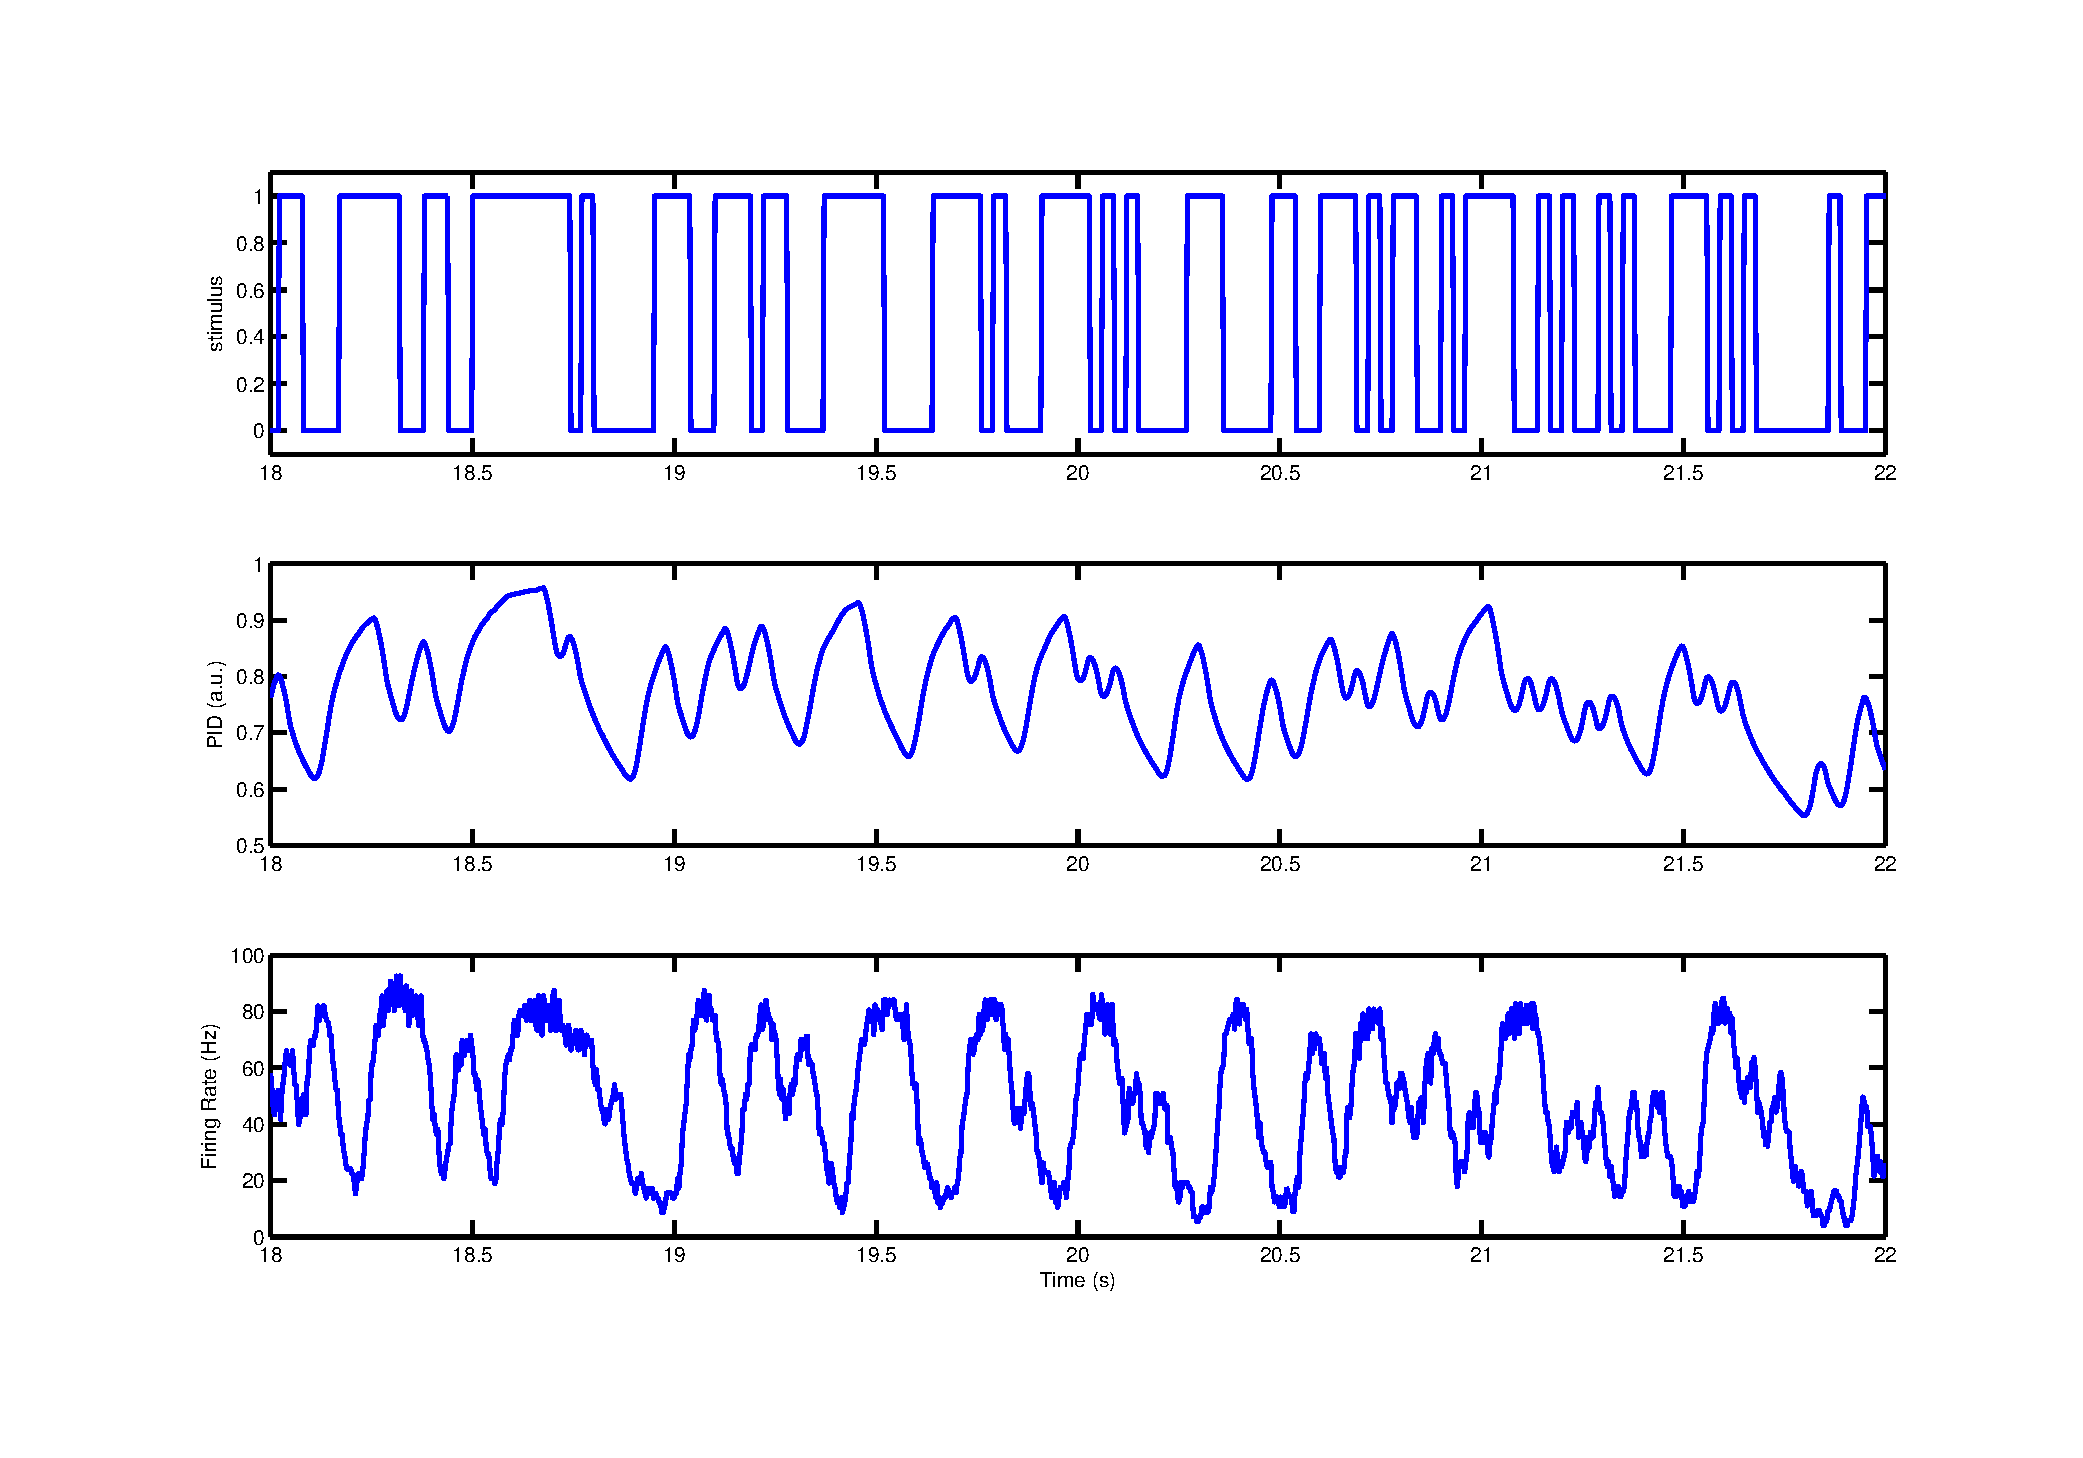
\includegraphics [width=\textwidth]{Analysis_January_01.pdf}
\begin{par}
The odour used, the neuron recorded from and the correlation time of the flickering stimulus are in the file name displayed above the plot.
\end{par} \vspace{1em}


\subsection*{Filter Extraction}

\begin{par}
Now, we extract a simple linear filter from the stimulus such that a convolution with the input (stimulus) gives the output (ORN firing rate).
\end{par} \vspace{1em}
\begin{par}
The filter is calculated using Chichilnisky's method. The only modification I have used is to regularise the matrix before inversion. The code is based on what Carlotta uses, and I have re-written it for clarity and modified the regularisation step.
\end{par} \vspace{1em}
\begin{par}
The filter \textit{K} is given by
\end{par} \vspace{1em}
\begin{par}
$$ C*K=s'*f $$
\end{par} \vspace{1em}
\begin{par}
where C is
\end{par} \vspace{1em}
\begin{par}
$$ C=\mathrm{Cov}(s)+\frac{rI}{1+r} $$
\end{par} \vspace{1em}
\begin{par}
where \textit{I} is the identity matrix and \textit{r} is a free parameter called the regularisation factor that suppresses the high-frequency components of \textit{K}. \textit{s} is the stimulus vector (e.g. the PID) and \textit{f} is the response vector (here, the firing rate of the ORN). In practice, \textit{K} is estimated by a left matrix division:
\end{par} \vspace{1em}
\begin{par}
$$ K=C\setminus(s'*f) $$
\end{par} \vspace{1em}
\begin{par}
For comparison, I have also calculated the filter using Damon's function (Back\_out\_1dfilter\_new)
\end{par} \vspace{1em}
\begin{par}
The problem of choosing \textit{r} appropriately remains. If \textit{r} is too low, then the effective number of parameters of the filter goes up, permitting over-fitting of the data, and you end up with a noisy squiggle of a filter that fits the data well. If \textit{r} is too high, the filter has too few modes, and doesn't fit the data well, but looks nice. The ideal \textit{r} is chosen so that it is equal to
\end{par} \vspace{1em}
\begin{par}
$$ \arg\min_{r}\left\Vert \frac{e(r)-\min(e)}{\min(e)},\frac{S(r)-\min(S)}{\min(S)},\frac{\left|m(r)-1\right|}{1}\right\Vert _{\infty} $$
\end{par} \vspace{1em}
\begin{par}
where \textit{e} is the error of the prediction w.r.t to the actual data, \textit{S} is the absolute sum of the filter \textit{K}, and \textit{m} is the slope of the best fit of the prediction to the data. Minimising \textit{e} minimises the error of the fit. Minimising \textit{S} minimises the high-frequency components in the filter, and prevents over-fitting. We also want the slope \textit{m} to be as close to 1 as possible.
\end{par} \vspace{1em}
\begin{par}
For a detailed look at how the slope of best fit and the filter shape vary with \textit{r}, look at the next section.
\end{par} \vspace{1em}
\begin{par}
In the figure below, the filter computed the PID and the firing rate is shown. In blue is the filter calculated using Chichilnisky's method, and in red is the filter calculated using Damon's function. The x axis is the lag of the filter, and the Y axis is the amplitude of the filter (in Hz)
\end{par} \vspace{1em}

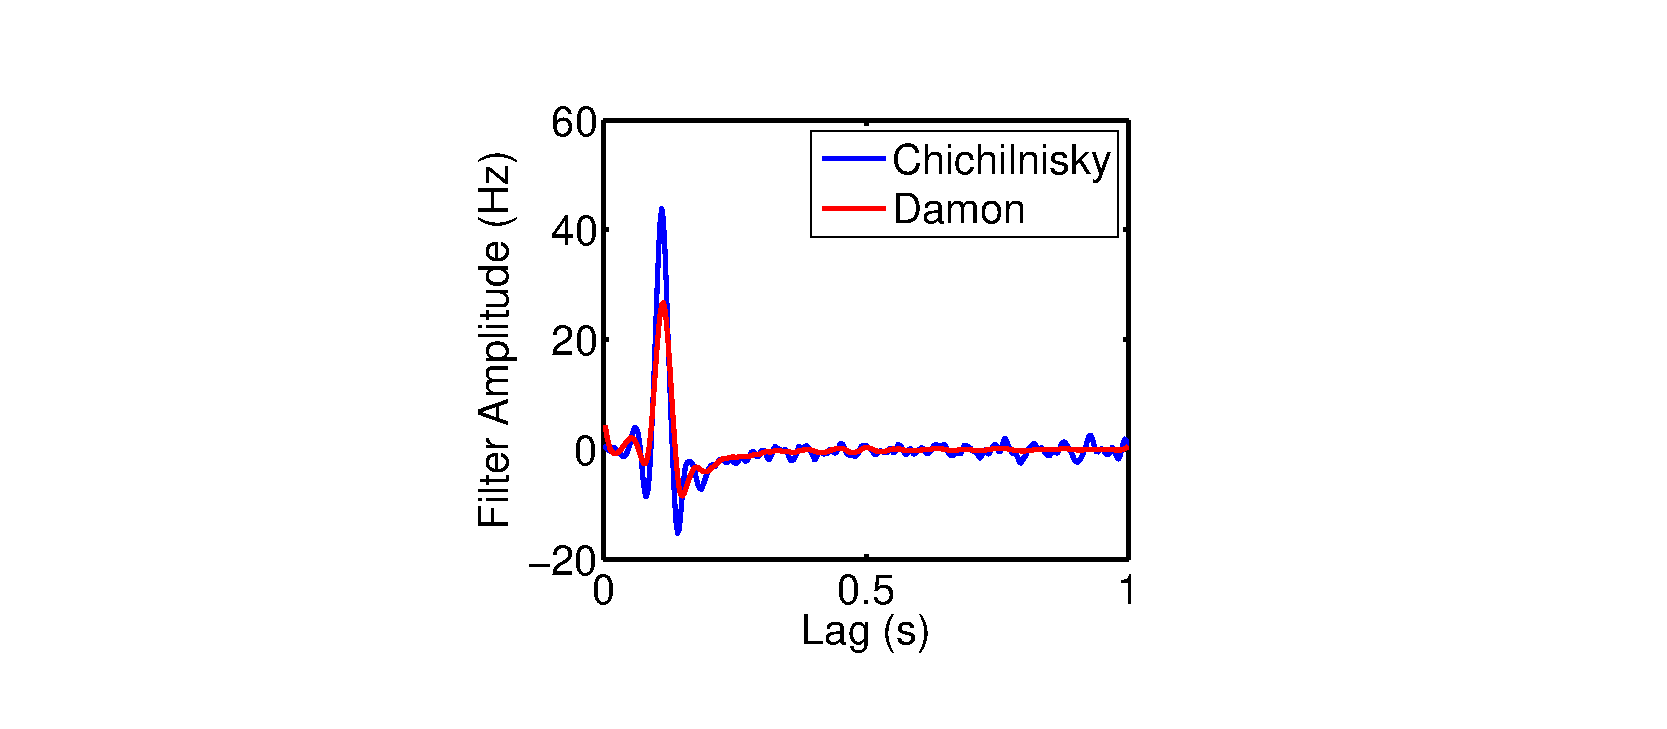
\includegraphics [width=\textwidth]{Analysis_January_02.pdf}
\begin{par}
The convolution of this filter with the input (PID) gives a prediction of the output. In the figure below, the data is shown in black, and the prediction from this linear filter is shown in blue (Chichilnisky method) and red (Damon's function). Note that sometimes the prediction is below zero, which doesn't mean anything physical (firing rate cannot be \ensuremath{<} 0).
\end{par} \vspace{1em}

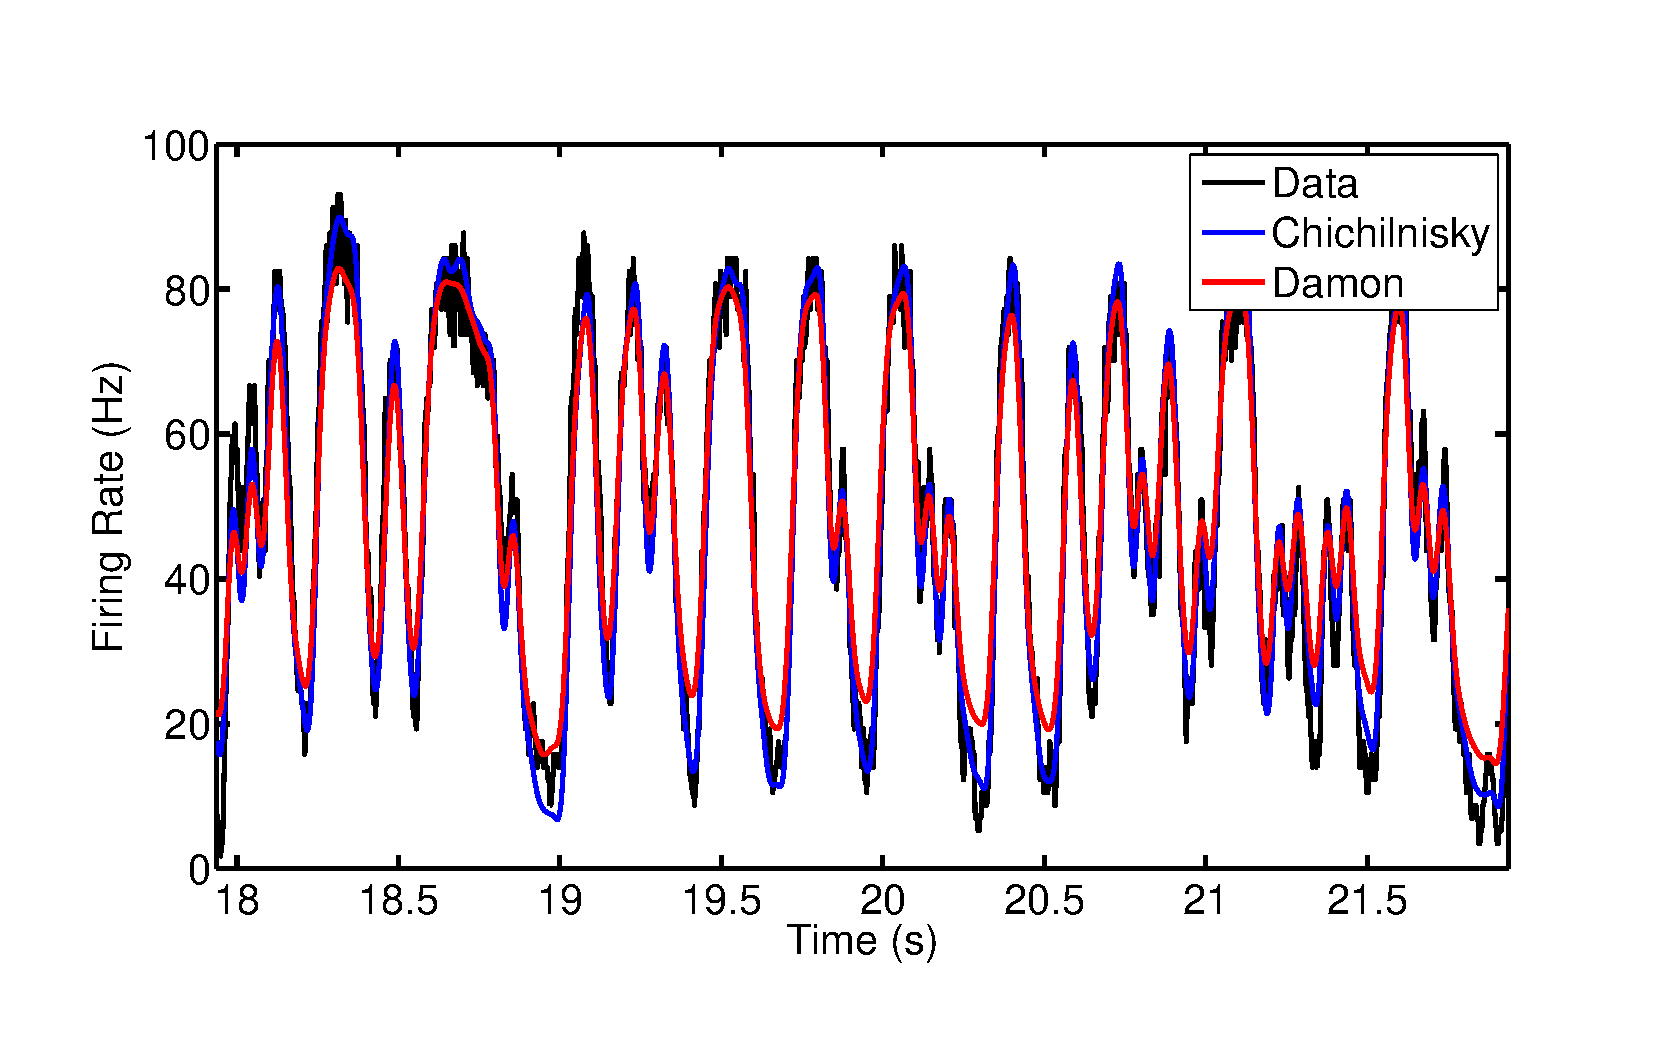
\includegraphics [width=\textwidth]{Analysis_January_03.pdf}


\subsection*{Analysis of Linear Prediction - Linearity of Prediction}

\begin{par}
For a linear filter calculated from the data, a plot of the actual response to the predicted response can be fit with a line of slope 1. Here the actual firing rate is plotted on the X axis and the firing rate predicted from the linear filter is plotted on the Y axis.
\end{par} \vspace{1em}

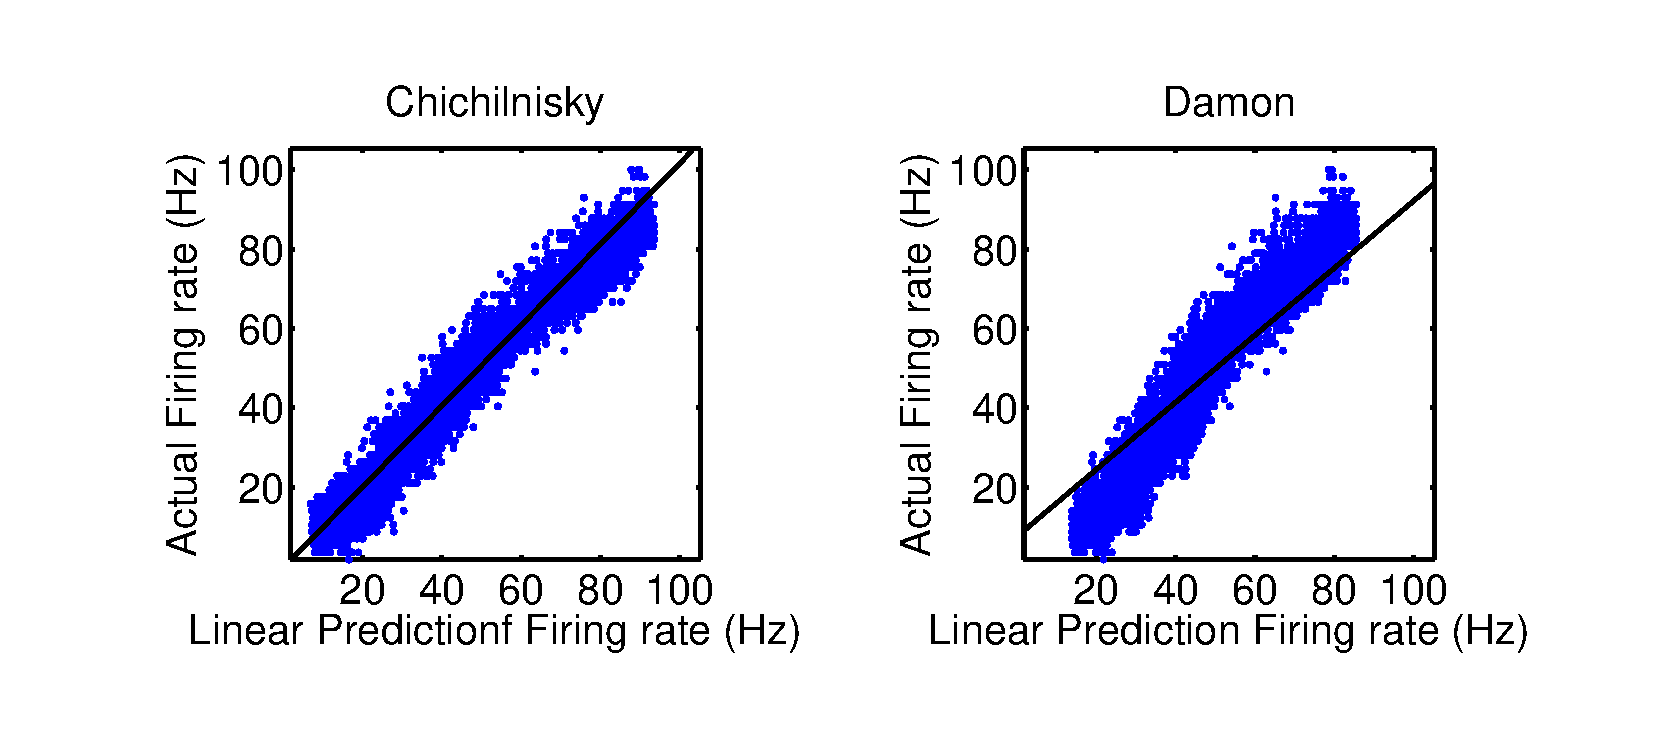
\includegraphics [width=\textwidth]{Analysis_January_04.pdf}
\begin{par}
The line is a best fit to all the data. The slope of the best fit line to Chichilnisky's fit is:
\end{par} \vspace{1em}

        \color{lightgray} \begin{verbatim}    0.9804

\end{verbatim} \color{black}
    \begin{par}
The line is a best fit to all the data. The slope of the best fit line to Damon's fit is:
\end{par} \vspace{1em}

        \color{lightgray} \begin{verbatim}    1.1819

\end{verbatim} \color{black}
    \begin{par}
Both Damon's and my filter estimation functions have a free parameter, \textit{r}, the regularisation factor. The following plots show how the error, the filter sum, and the filter height vary with varying the free parameter \textit{r}. The point in red indicates the value of \textit{r} finally chosen for the best filter. Note that for the Chichilnisky filter, the slope is very close to 1. For very little regularisation, the slope is exactly 1.
\end{par} \vspace{1em}

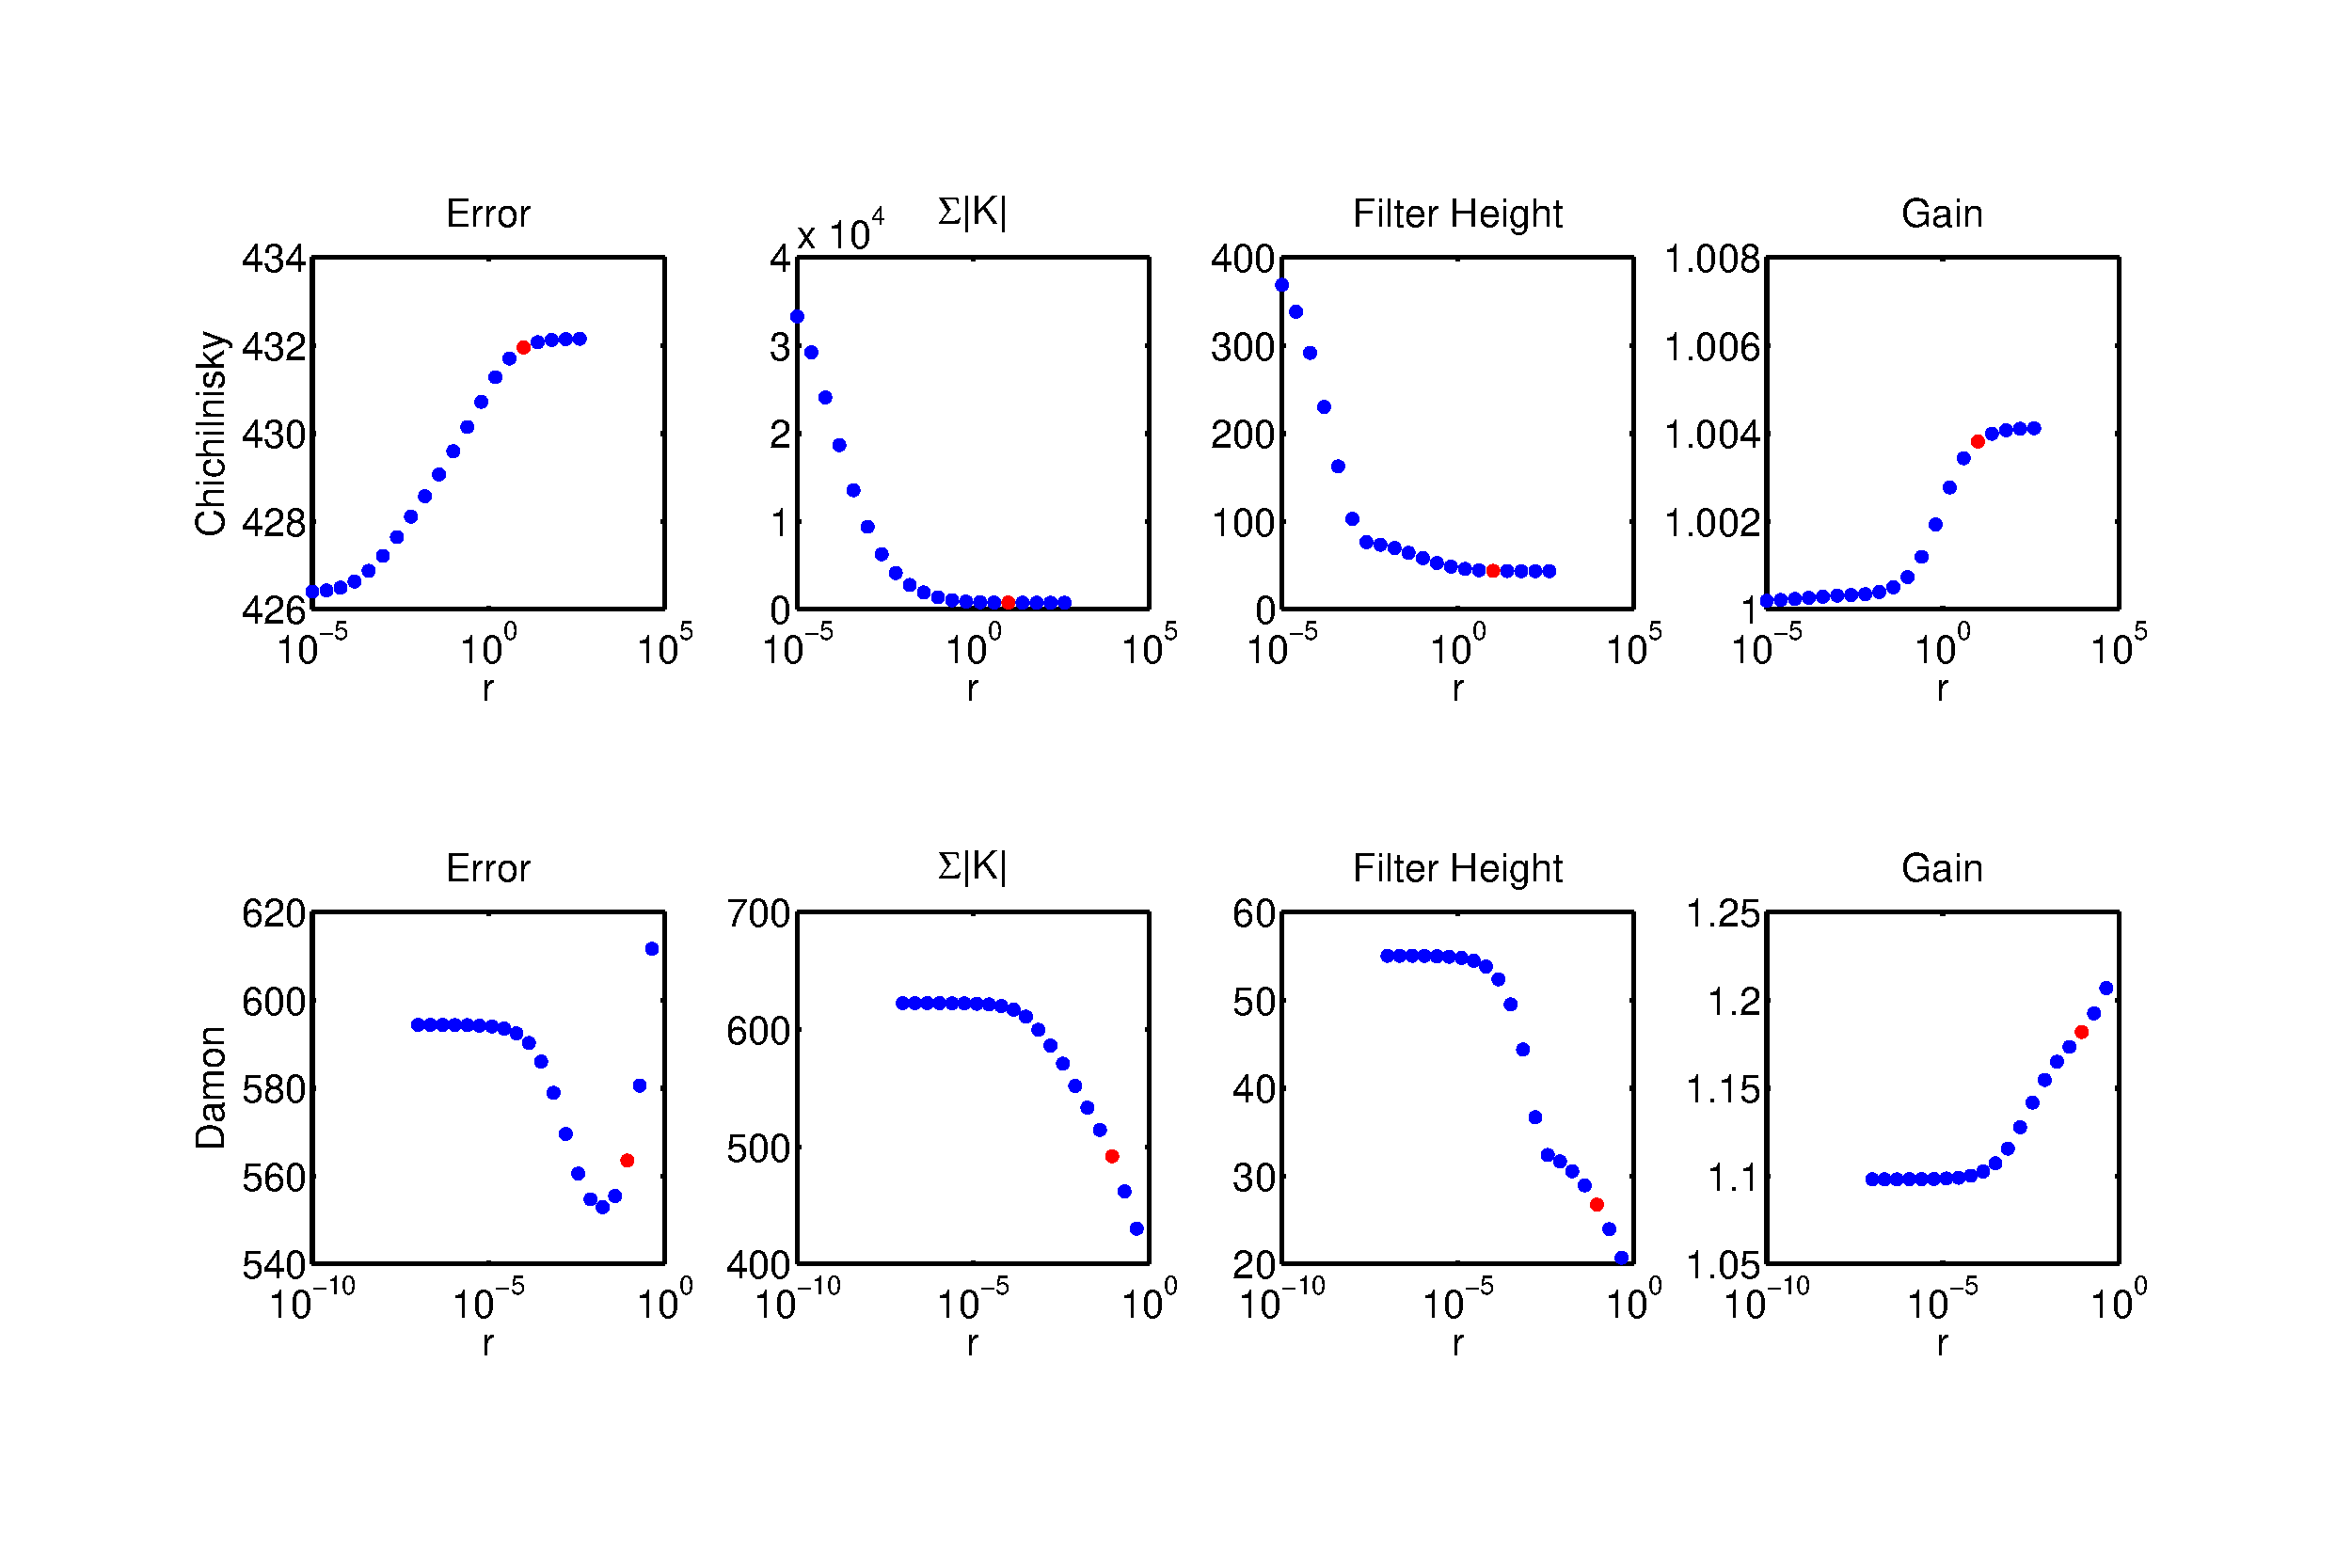
\includegraphics [width=\textwidth]{Analysis_January_05.pdf}


\subsection*{Analysis of Linear Prediction - Which input predicts output better?}

\begin{par}
The measurement of the stimulus should help us predict the response of the neuron better than just the valve control signal, as we now capture the fast fluctuations of the odour stimulus as it reaches the ORN. Thus, a prediction of ORN firing response from the PID signal should be better than a prediction of the ORN firing response from the valve signal.
\end{par} \vspace{1em}
\begin{par}
First, we recalculate a new filter from the valve control signal and the ORN firing rate using the same methods as before. The plot below shows this new filter:
\end{par} \vspace{1em}

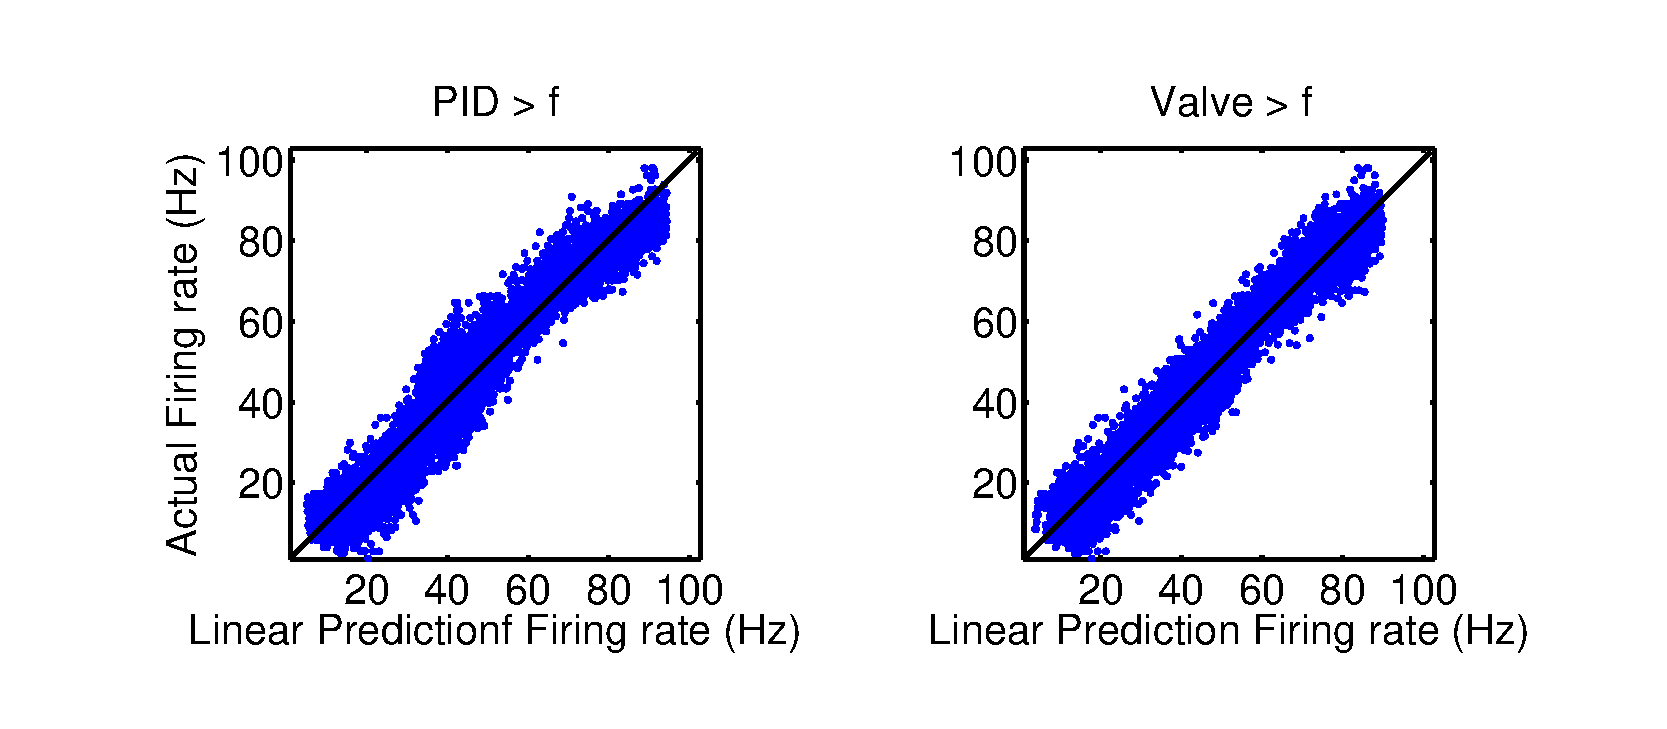
\includegraphics [width=\textwidth]{Analysis_January_06.pdf}
\begin{par}
As before, we can look at how changing \textit{r} changes the valve shape.
\end{par} \vspace{1em}

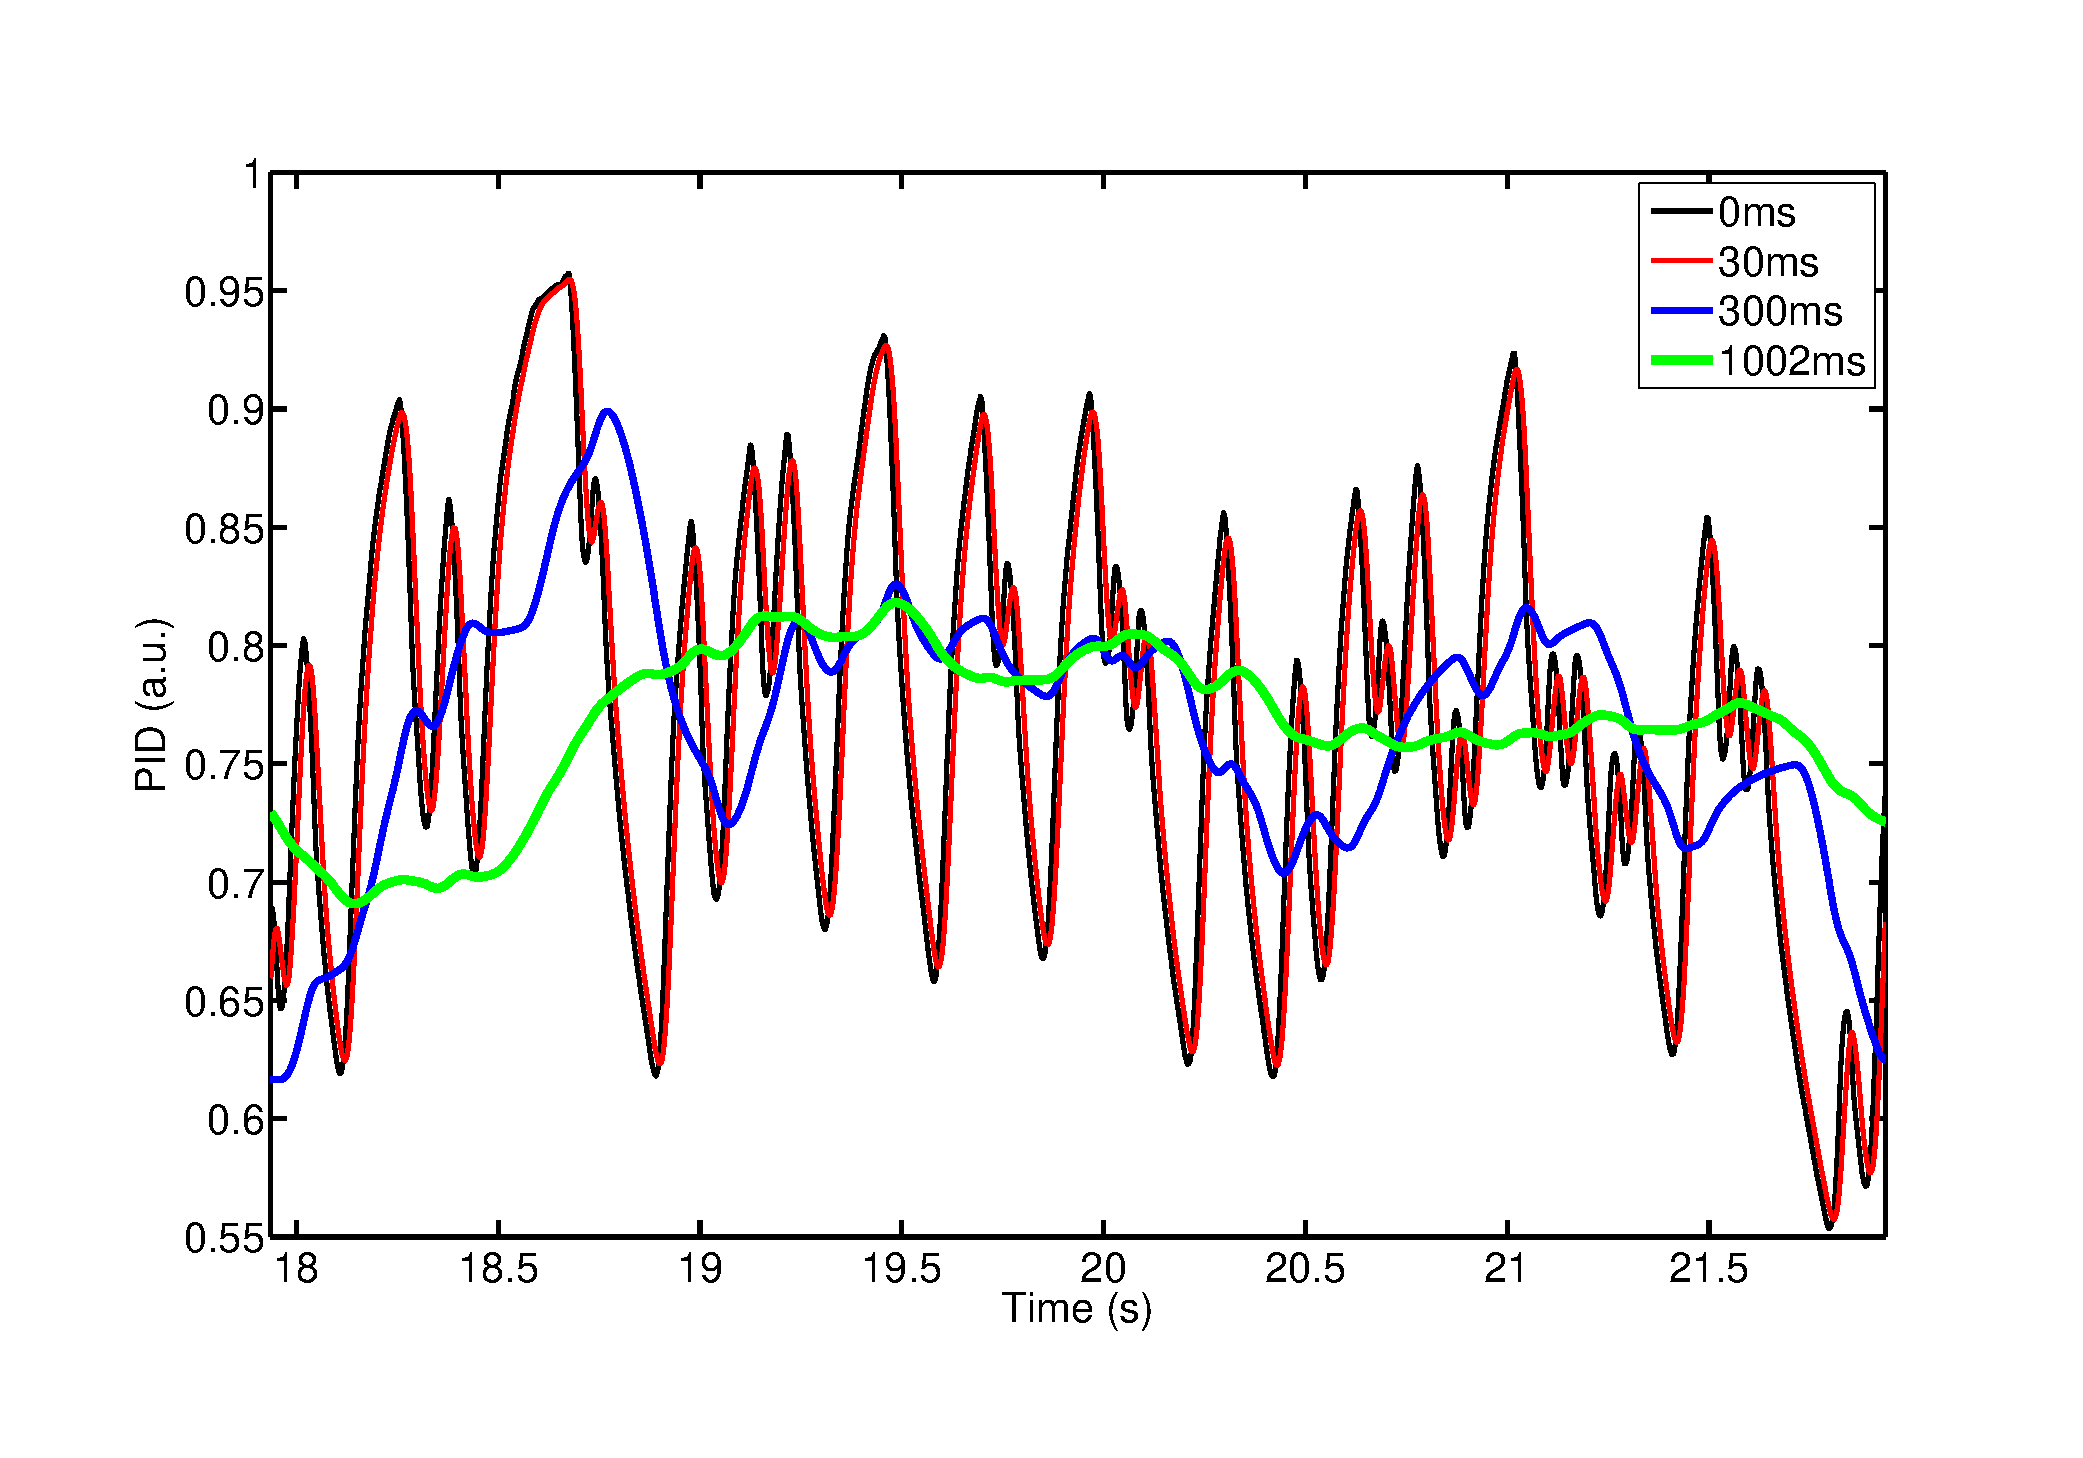
\includegraphics [width=\textwidth]{Analysis_January_07.pdf}
\begin{par}
Using the filter calculated using Damon's code, we make a new prediction of the firing rate of the ORN. In the figure below, the data is shown in blue, the linear prediction from the PID is shown again in red, and the linear prediction from the Valve is shown in black.
\end{par} \vspace{1em}

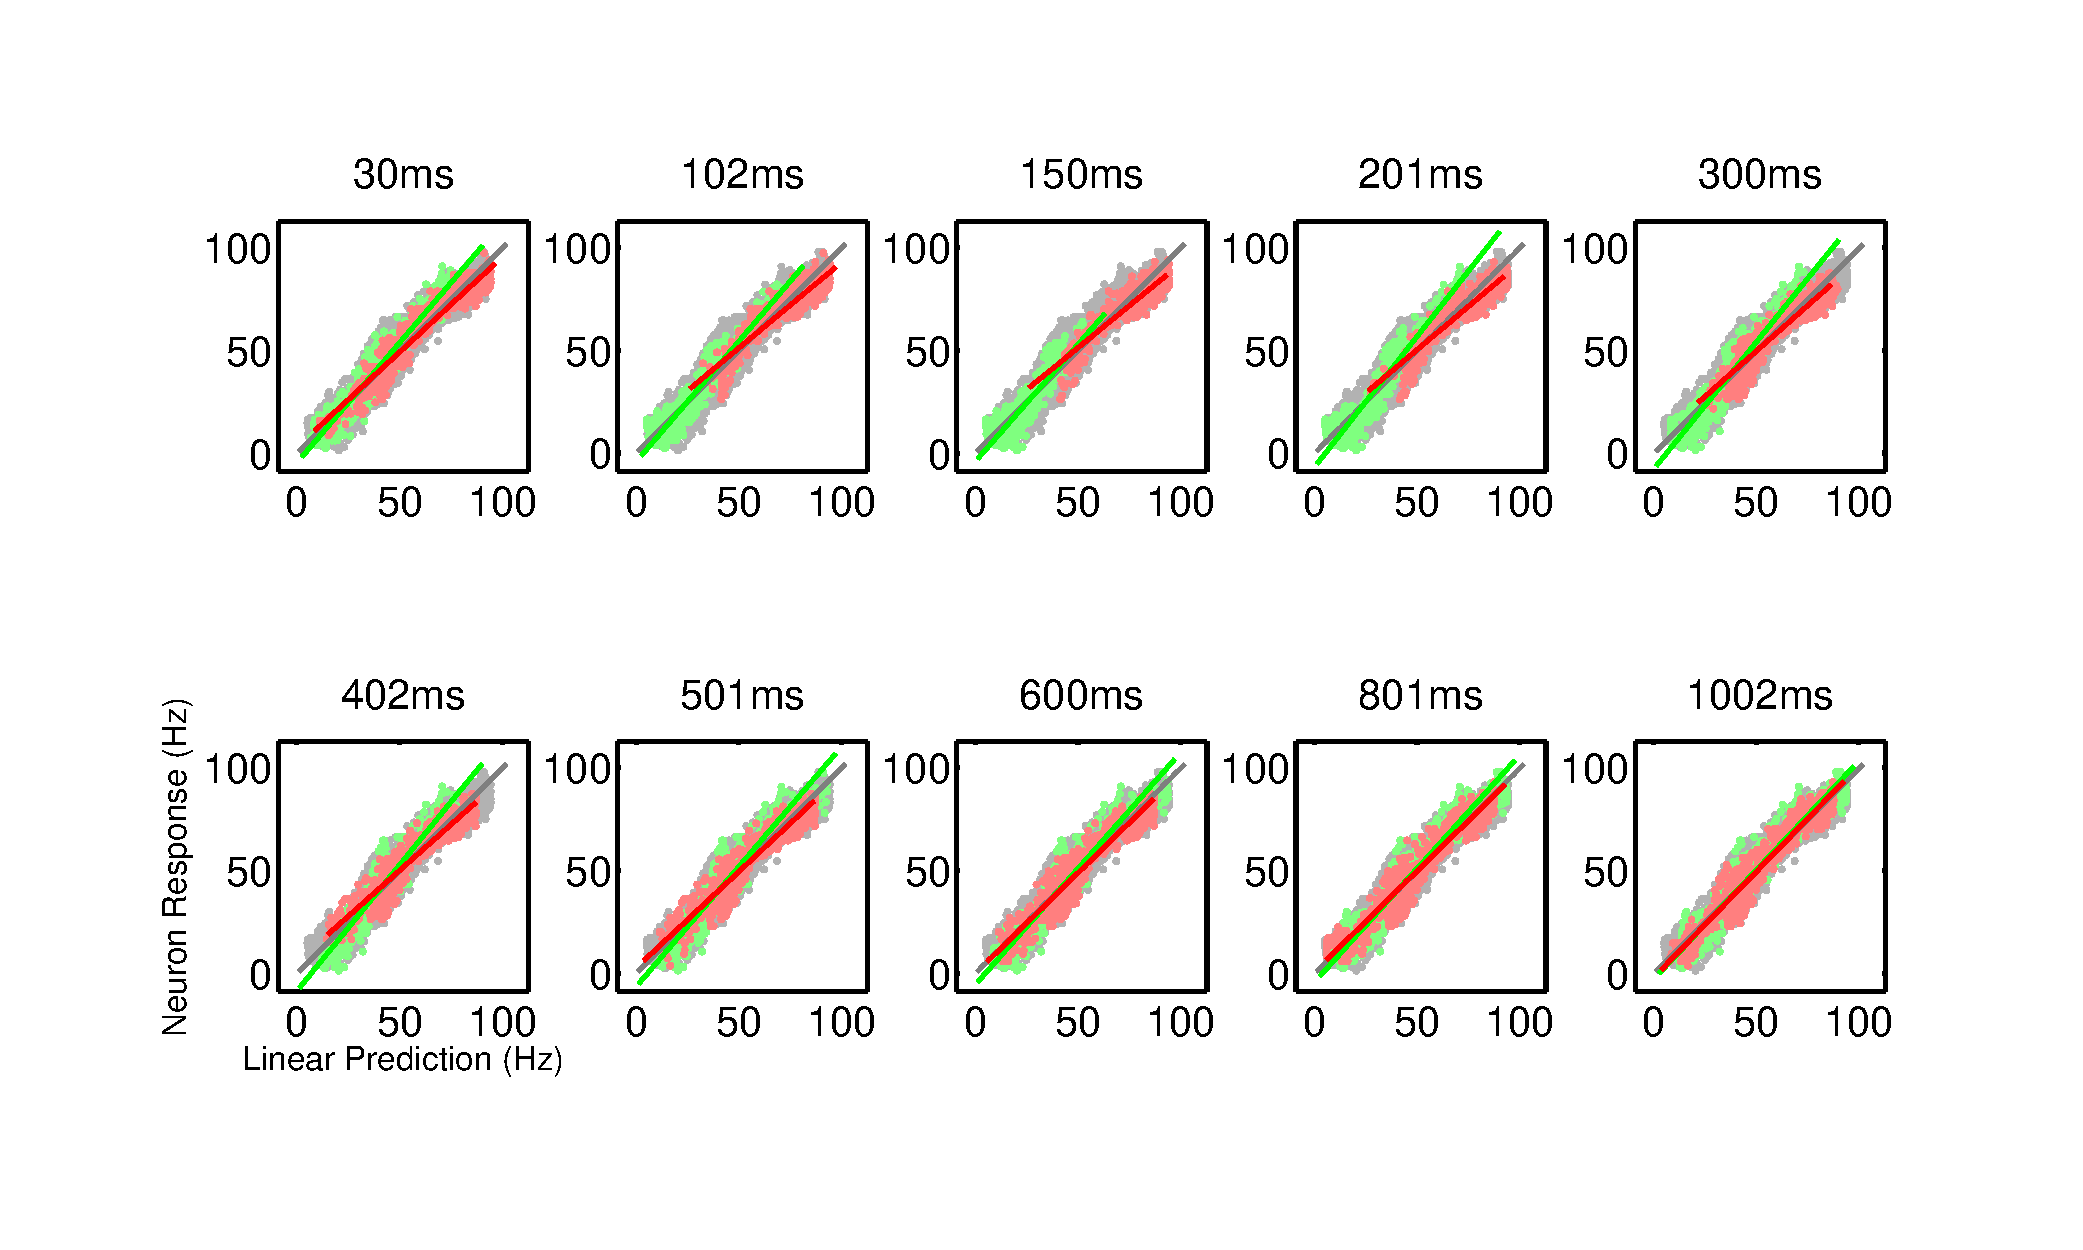
\includegraphics [width=\textwidth]{Analysis_January_08.pdf}
\begin{par}
The quality of the prediction is measured using the Root-mean-square error, calculated as:
\end{par} \vspace{1em}
\begin{par}
$$ \triangle t*\sqrt[]{\Sigma \left(f-f_{p}\right)^{2}} $$
\end{par} \vspace{1em}
\begin{par}
The error in the prediction from the PID, per unit time is:
\end{par} \vspace{1em}

        \color{lightgray} \begin{verbatim}    1.3089

\end{verbatim} \color{black}
    \begin{par}
while the error for the prediction from the Valve is:
\end{par} \vspace{1em}

        \color{lightgray} \begin{verbatim}    1.3955

\end{verbatim} \color{black}
    

\subsection*{Analysis of Linear Prediction - Response to High and Low Stimuli}

\begin{par}
How does the response of the ORN differ for high and low stimuli? Specifically, does the neuron display the characteristics of fast adaptation to this flickering stimulus?
\end{par} \vspace{1em}
\begin{par}
To look at this, we calculate the mean average stimulus over some window history length for every time point t, for various different window history lengths. The effect of this operation is shown in the figure below, where the legend refers to the history window in ms.
\end{par} \vspace{1em}

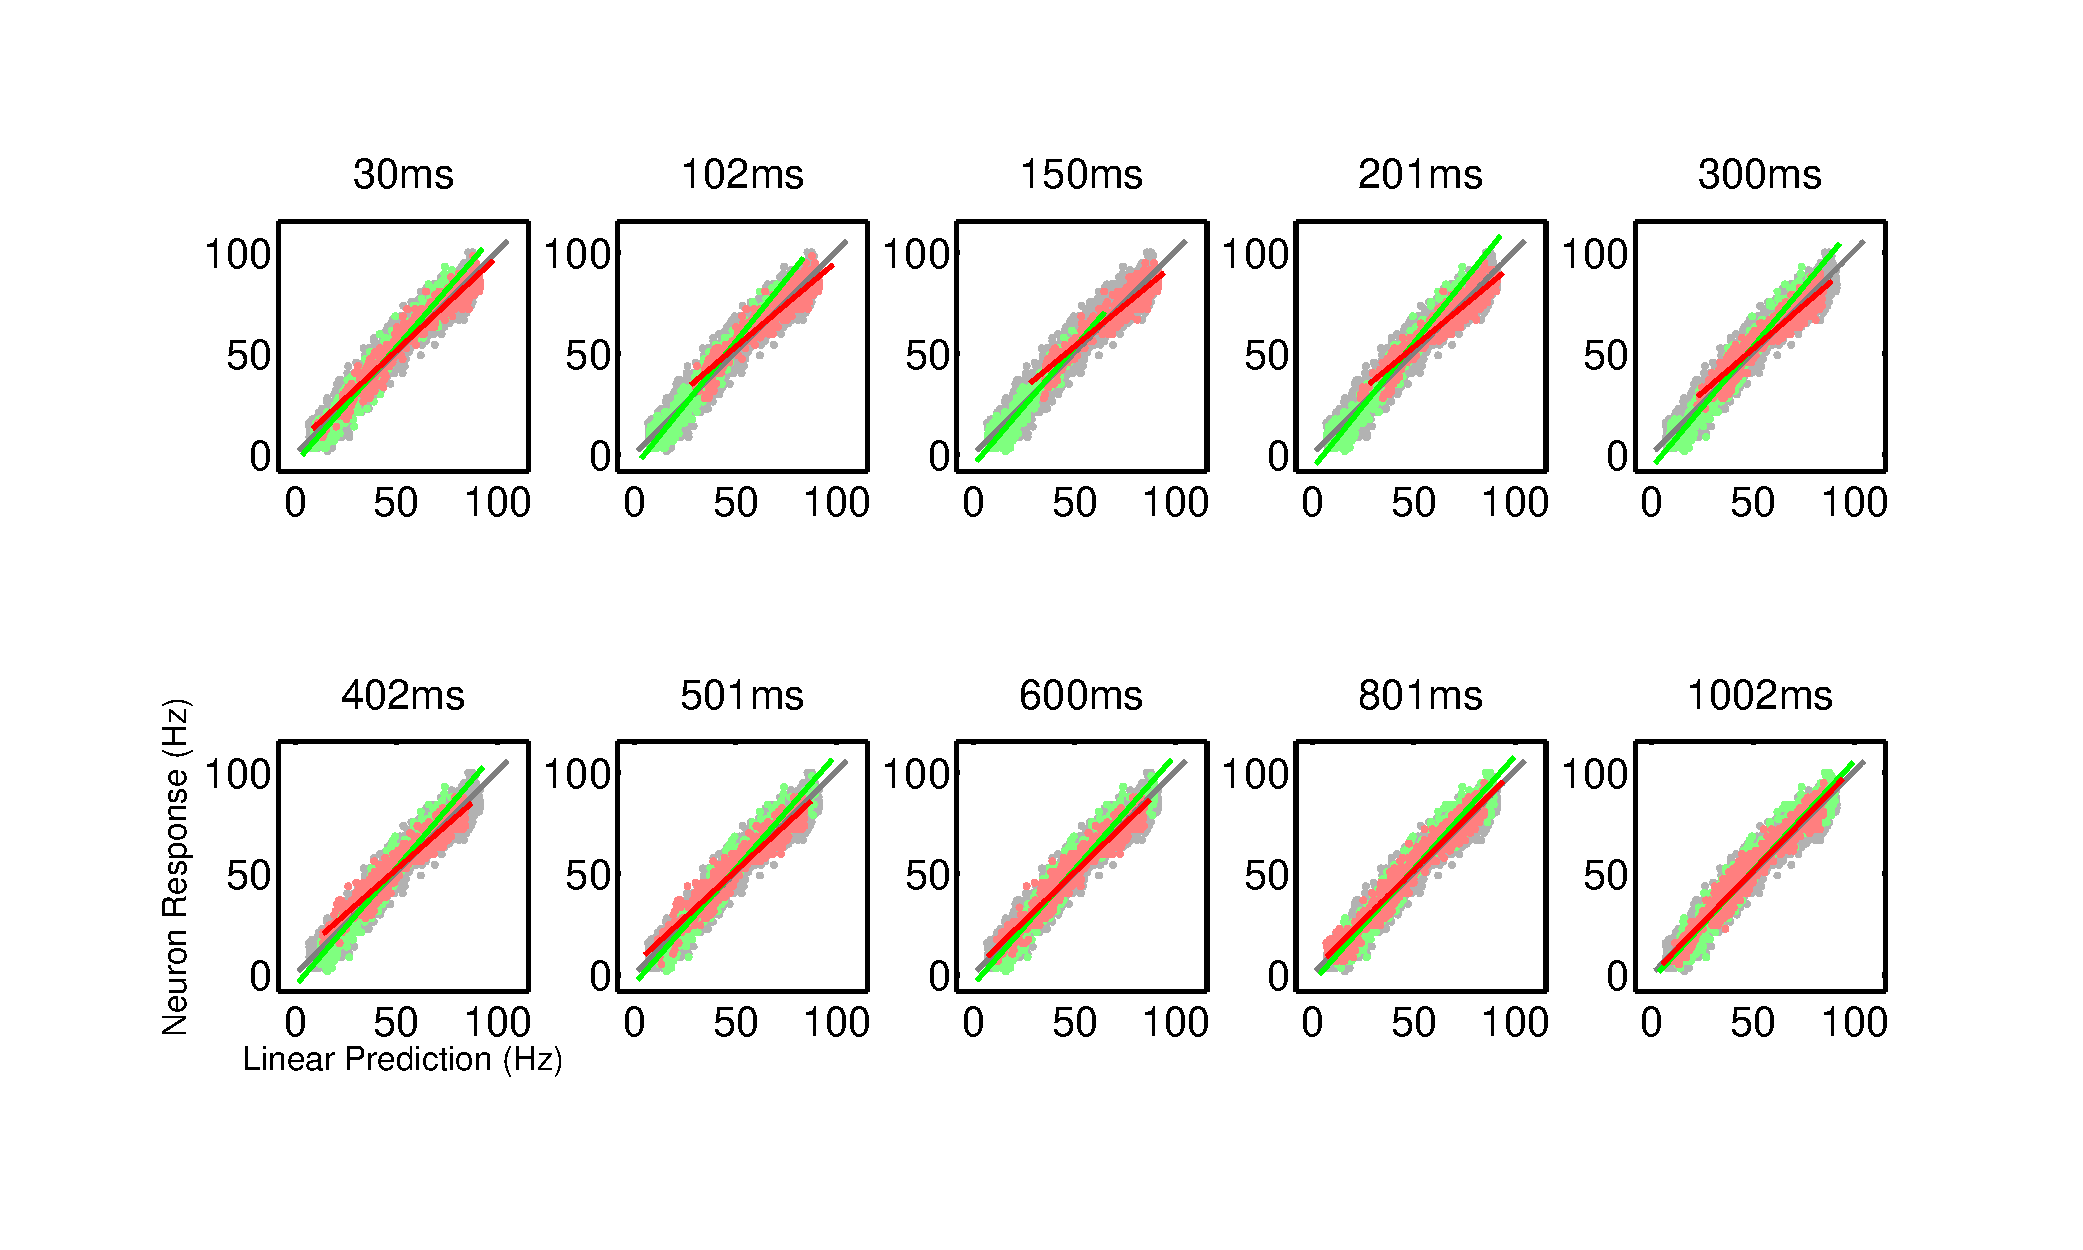
\includegraphics [width=\textwidth]{Analysis_January_09.pdf}
\begin{par}
Now, we separate neuron responses at times when the mean average stimulus is in the lowest 10\% or the highest 10\%. These points are marked either green (lowest 10\%) or red (or highest 10\%) in the figures below, while all the data is plotted in grey. Lines are fit to each of these clouds of points, and the slopes (representing the instantaneous gain) is calculated from these lines. The \textit{y} axis is the actual firing rate, while the \textit{x} axis is the predicted firing rate.
\end{par} \vspace{1em}

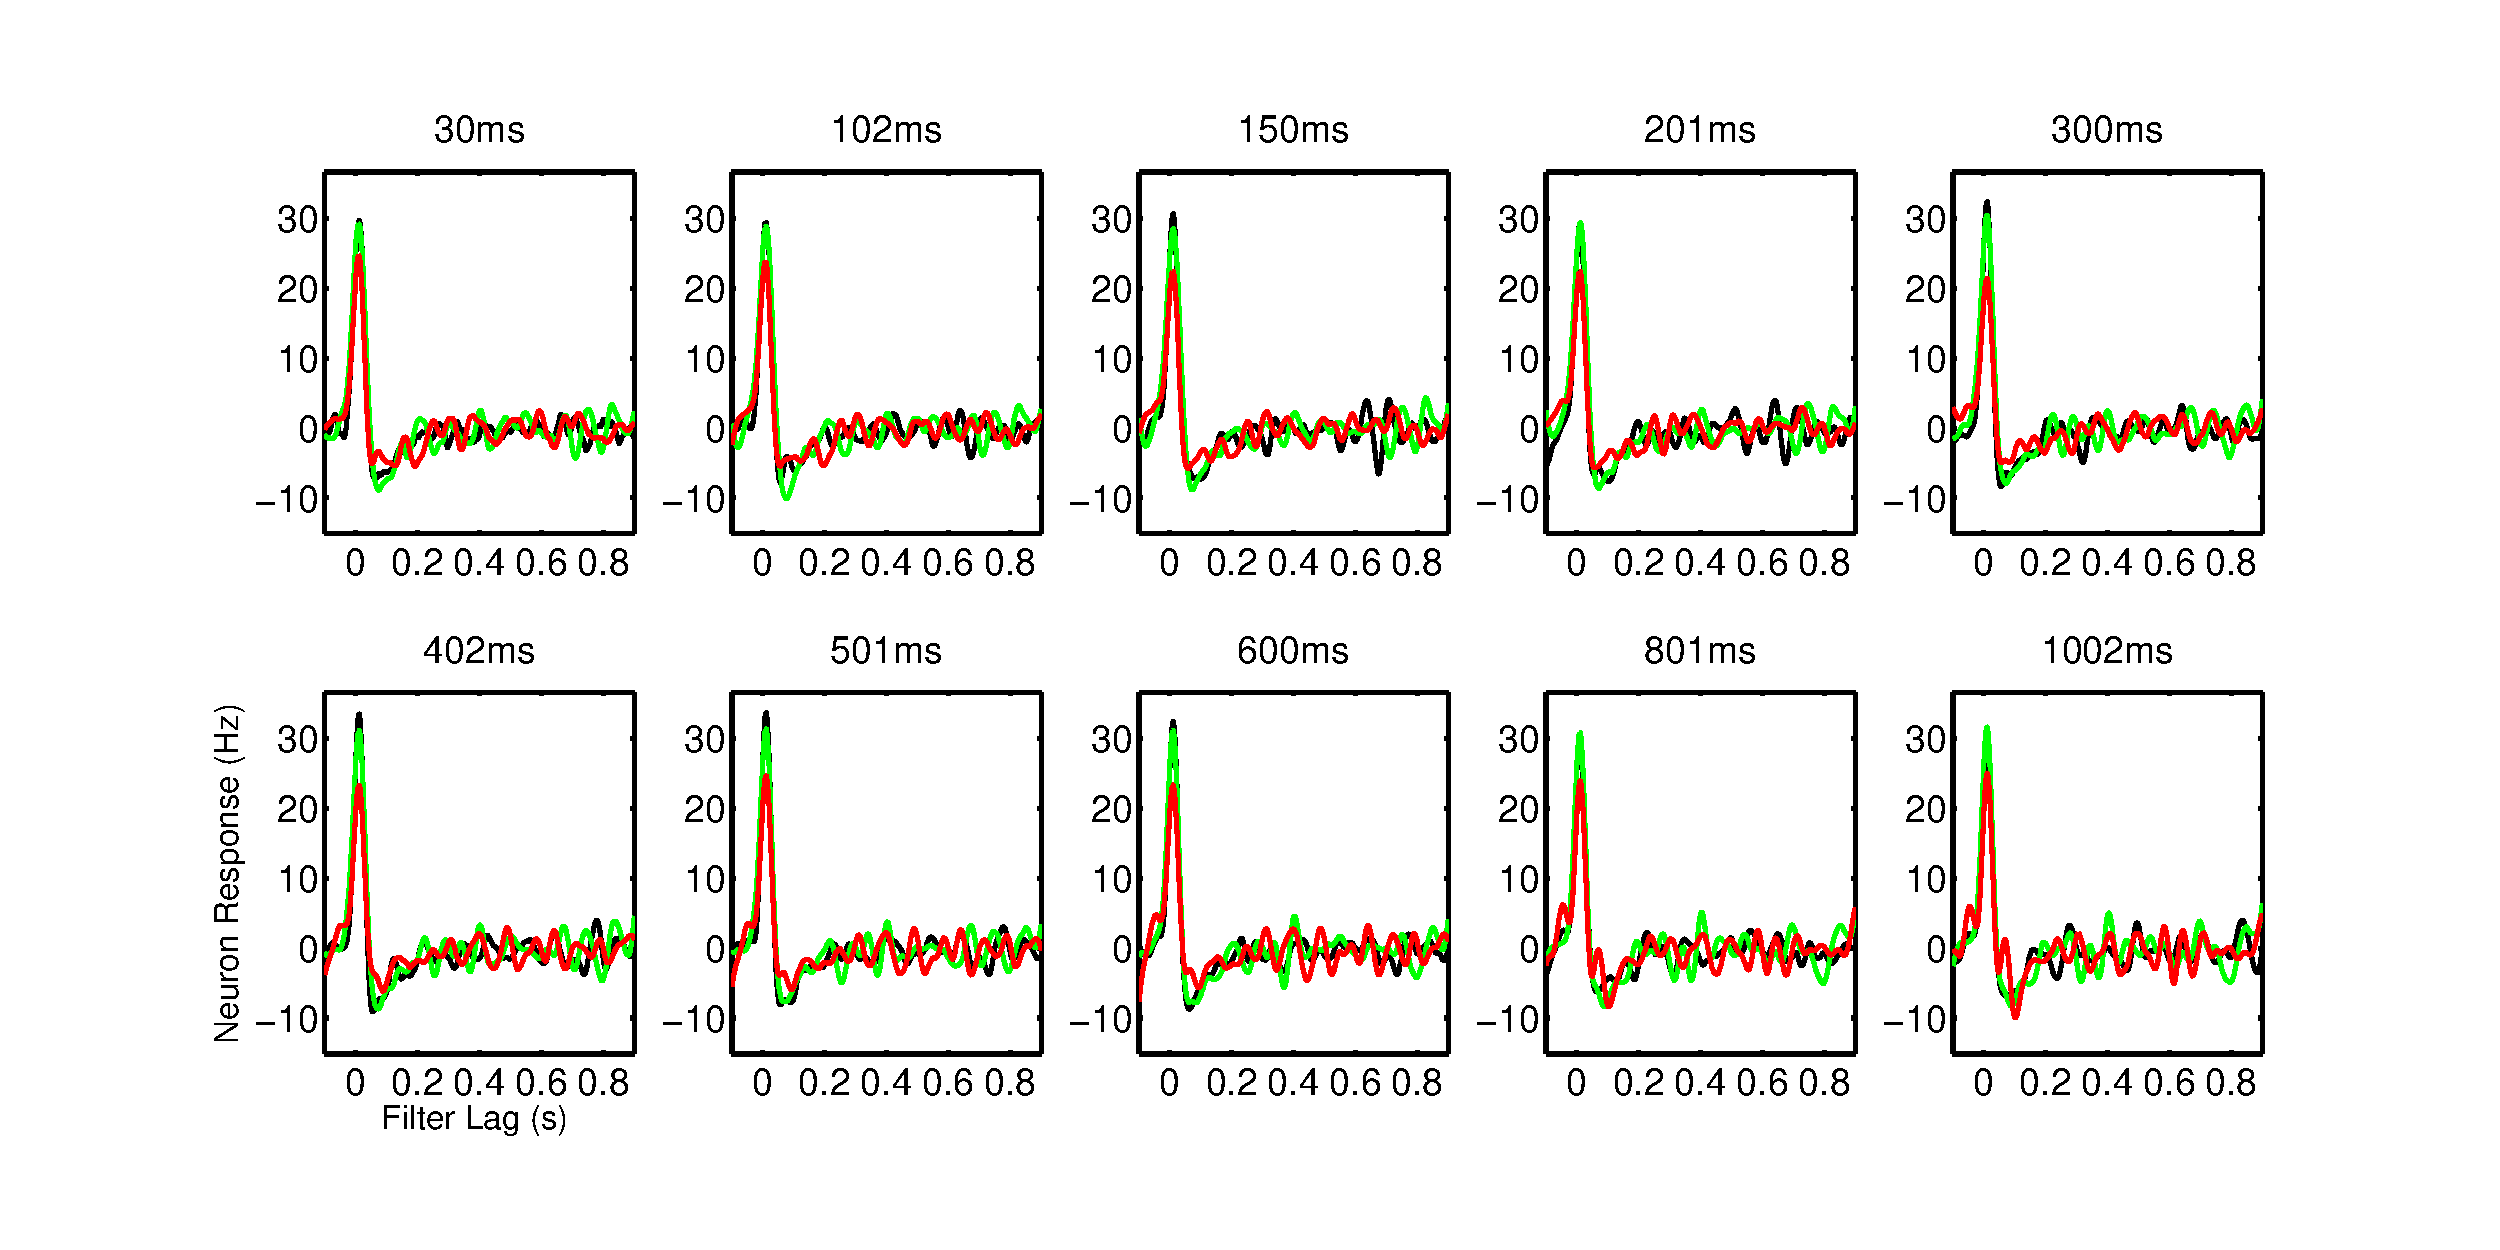
\includegraphics [width=\textwidth]{Analysis_January_10.pdf}
\begin{par}
The following plot shows how the slope of the lines of best fit, or the instantaneous gains, varies with the history length. The plot on the right shows the goodness of fit for each fit, indicating the regions where the fit is meaningful.
\end{par} \vspace{1em}

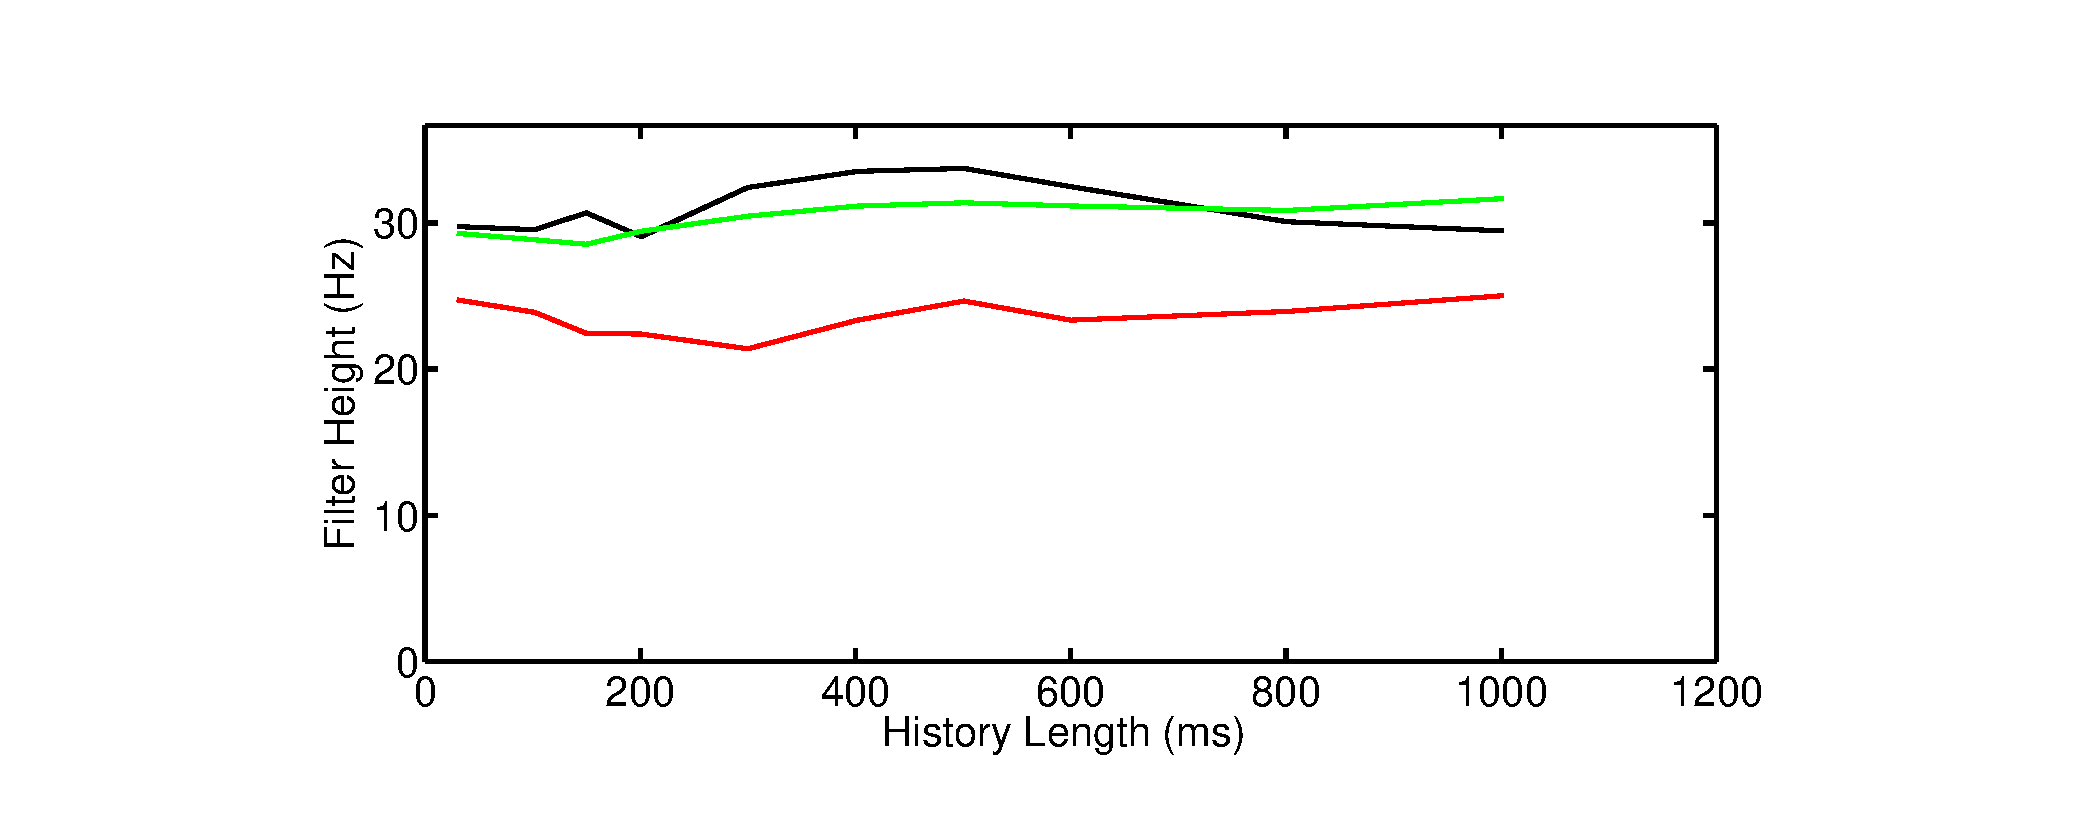
\includegraphics [width=\textwidth]{Analysis_January_11.pdf}


\subsection*{Analysis of Linear Prediction - Filter Variation}

\begin{par}
We have segmented the entire data set based on when the stimulus, averaged in some way over the past, into high and low. Here, I will calculate filters for each of these subsets.
\end{par} \vspace{1em}


\subsection*{Analysis of Linear Prediction -  Instantaneous Gain}

\begin{par}
There is a mismatch between the linear prediction and the actual firing rate. Moreover, the instantaneous gain seems to be modulated by something that depends on the past history of the stimulus. Here, in the figure below, the instantaneous gain, i.e., the ratio of the actual firing rate to the predicted firing rate, is plotted along with the stimulus.
\end{par} \vspace{1em}

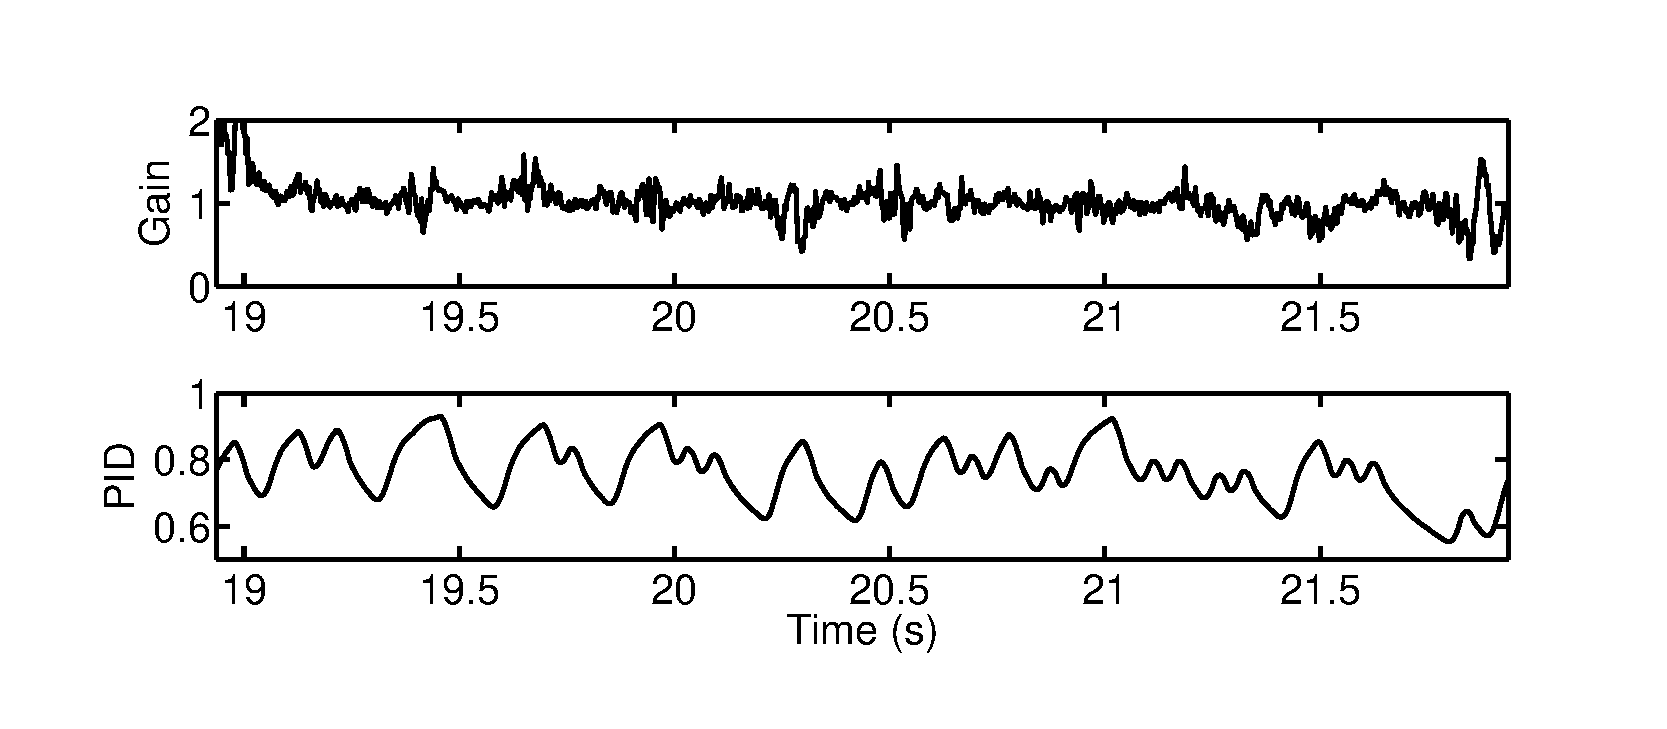
\includegraphics [width=\textwidth]{Analysis_January_12.pdf}
\begin{par}
In the above analysis, we have considered how a boxcar average over the stimulus immediately preceding the current time affects gain. Now, we want to find some optimal way of averaging the past stimulus history to predict the instantaneous gain: by doing so, we can then predict instantaneous gain, and thus get a better predictor of the actual firing rate.
\end{par} \vspace{1em}
\begin{par}
In effect, we can calculate a new filter, $K_g$ such that
\end{par} \vspace{1em}
\begin{par}
$$ K_g=C\setminus(s'*g) $$
\end{par} \vspace{1em}
\begin{par}
where \textit{g} is the instantaneous gain and \textit{s} is the stimulus.
\end{par} \vspace{1em}

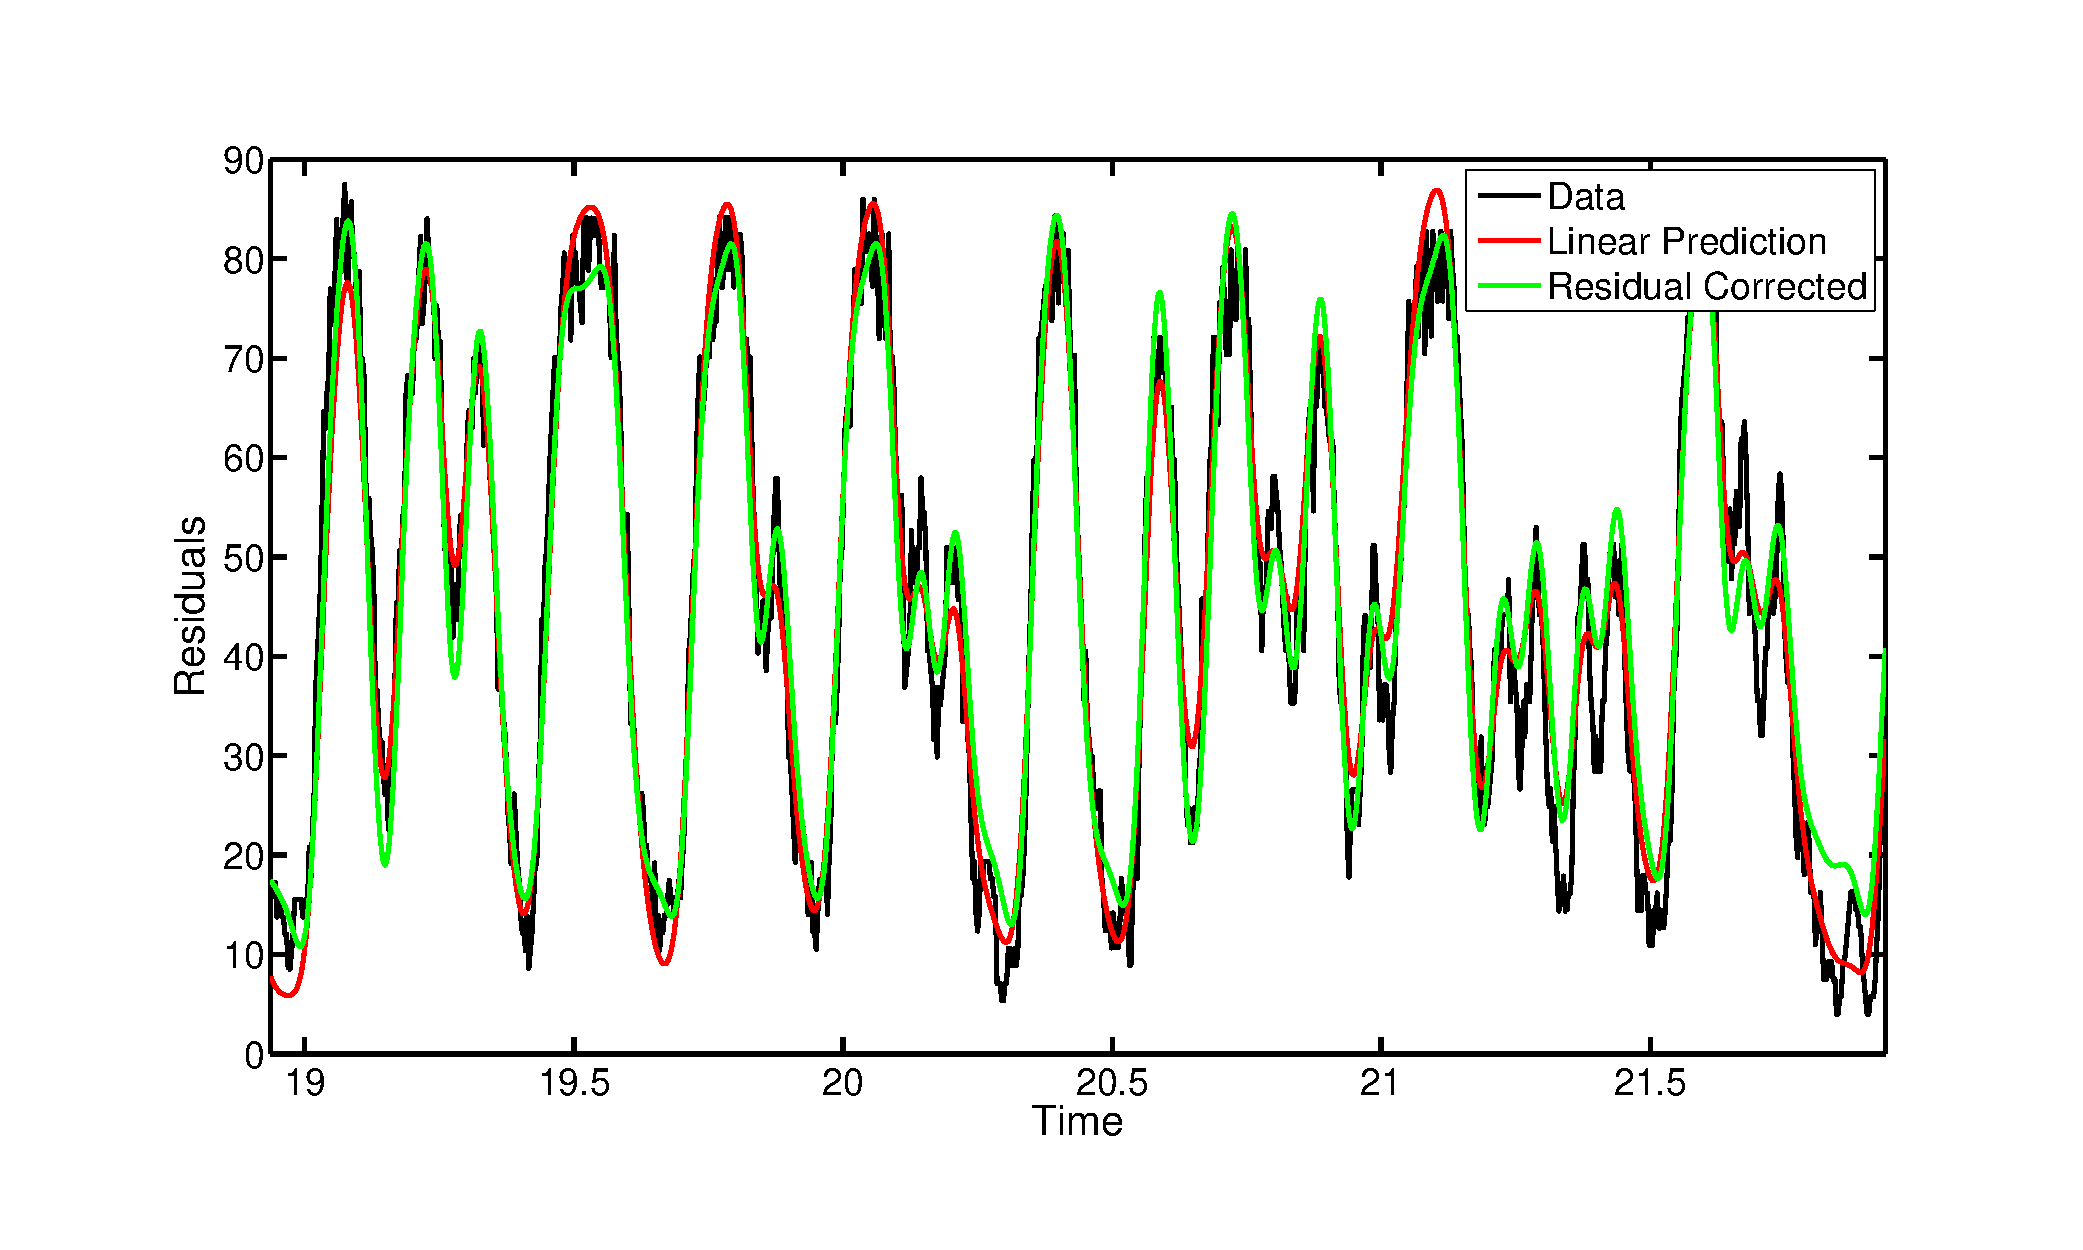
\includegraphics [width=\textwidth]{Analysis_January_13.pdf}
\begin{par}
Once again, we can vary the free parameter to see how to best choose a filter.
\end{par} \vspace{1em}

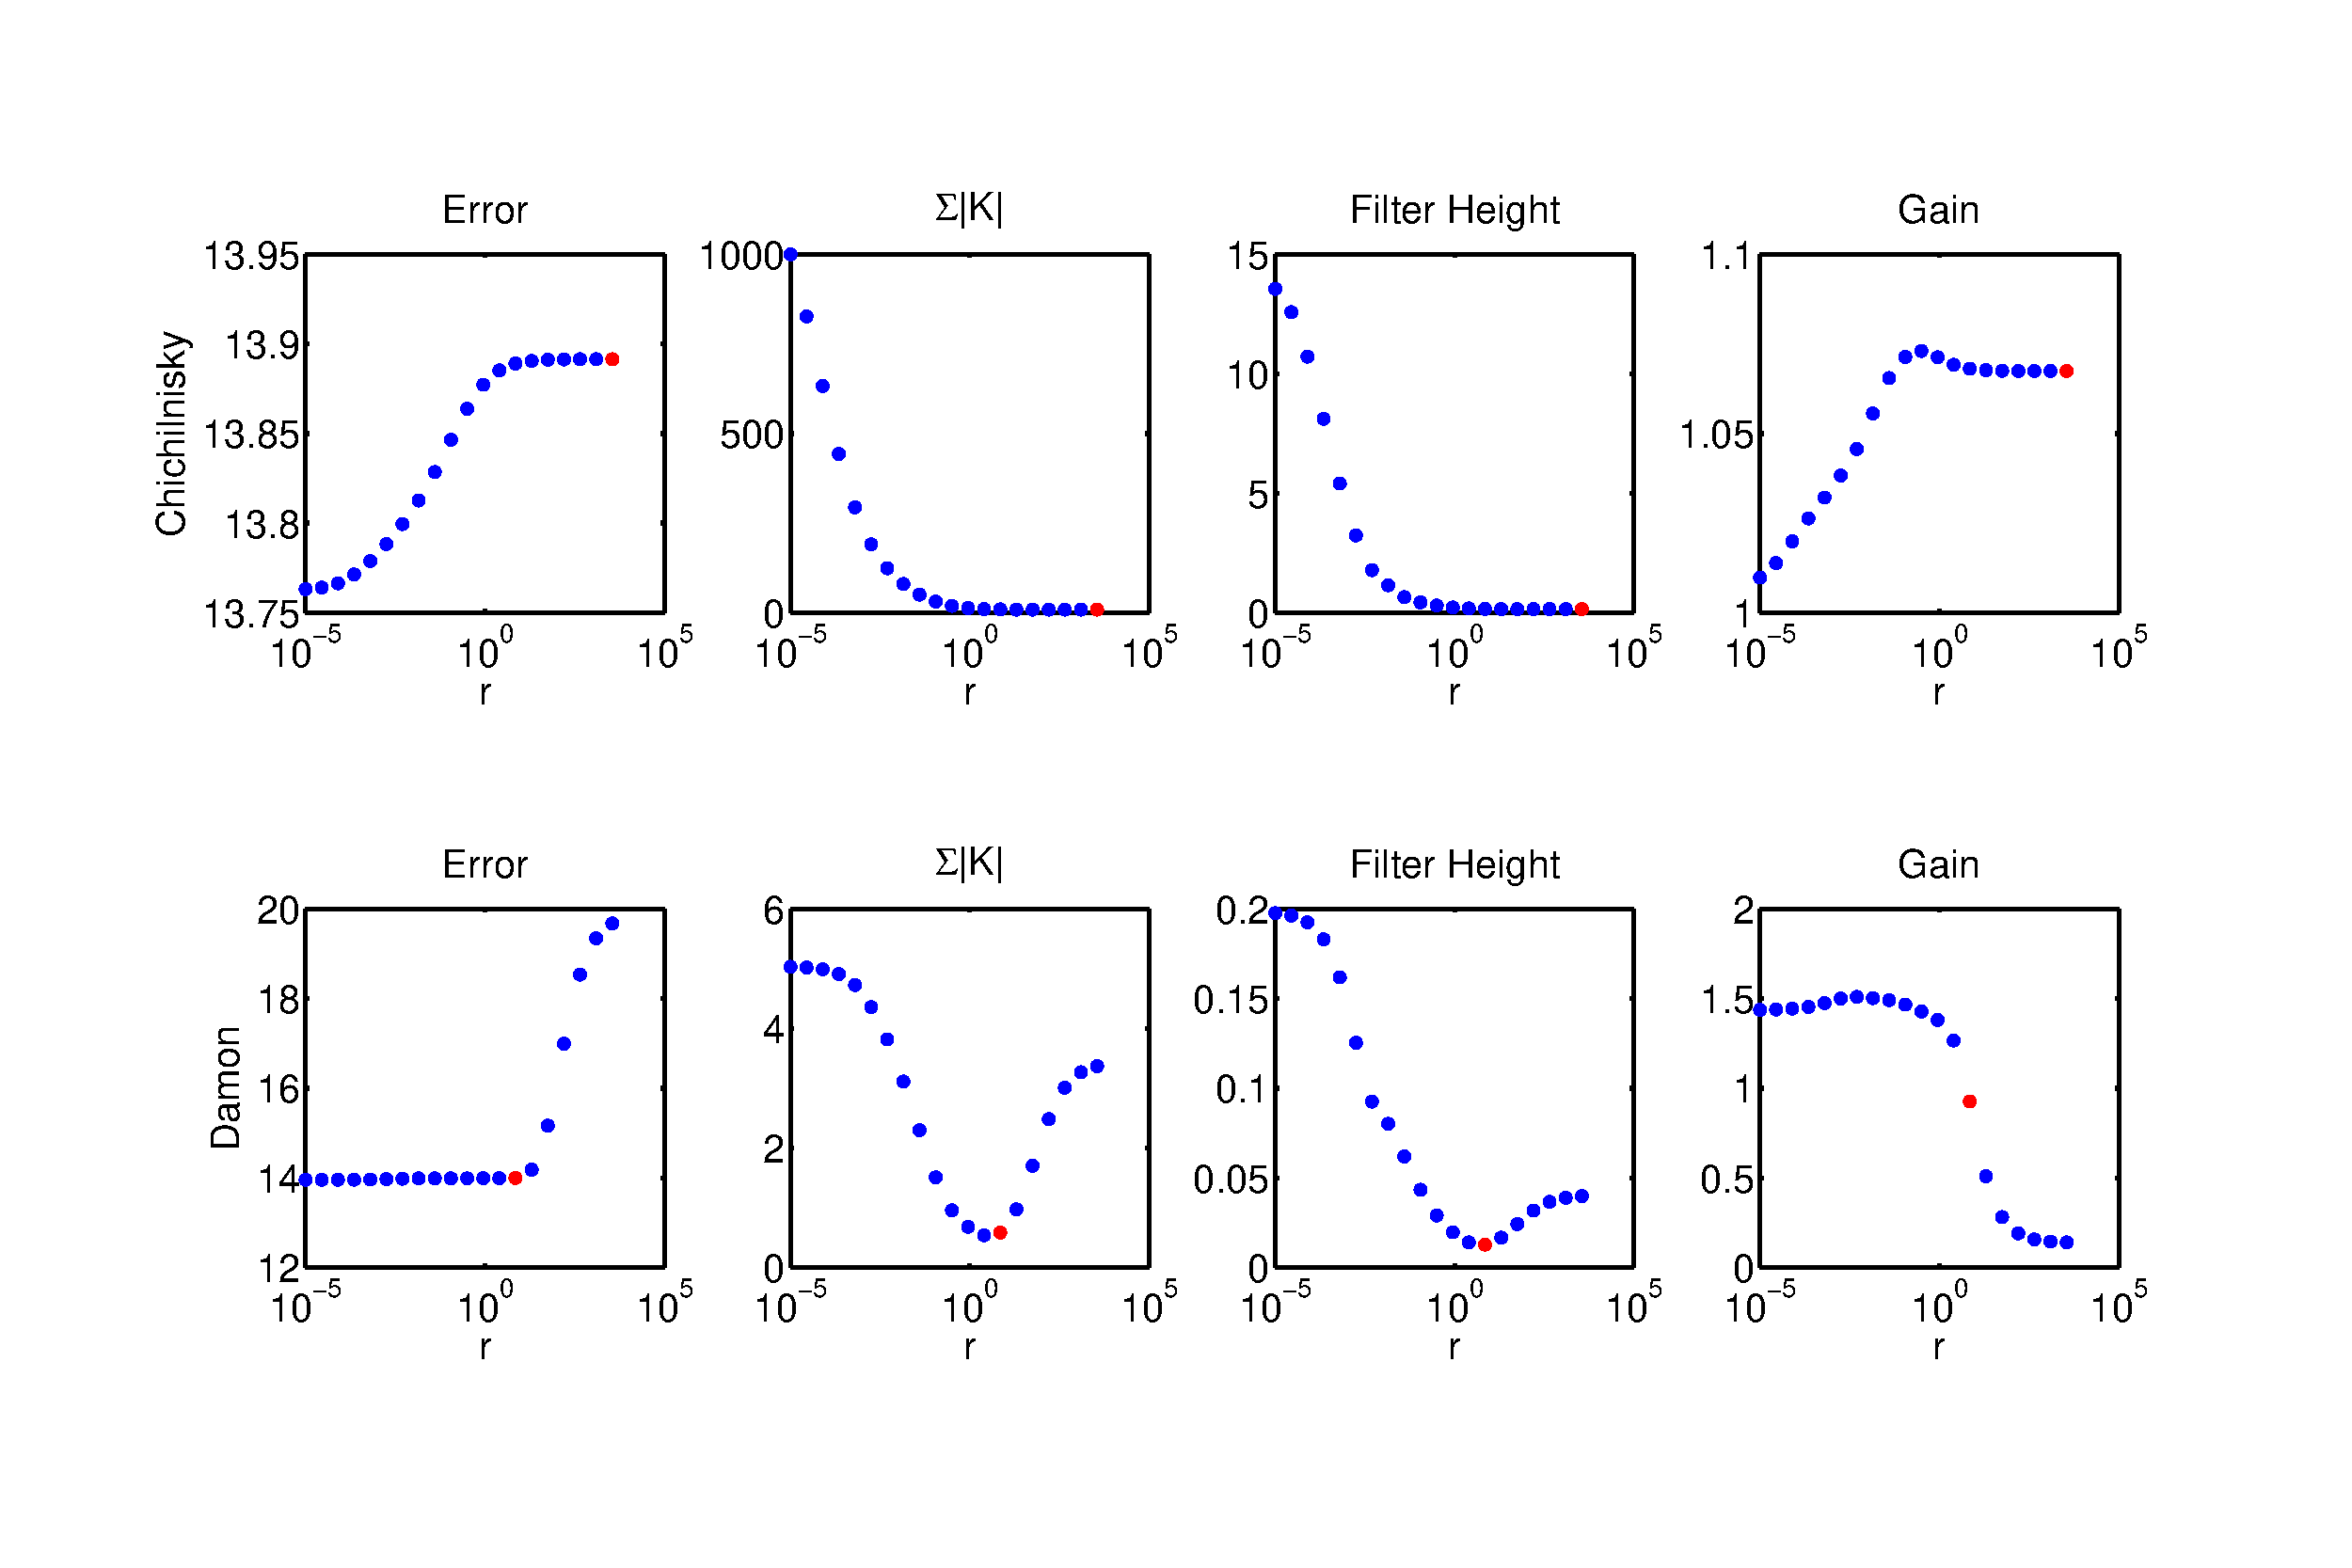
\includegraphics [width=\textwidth]{Analysis_January_14.pdf}
\begin{par}
From this filter and the stimulus, we can estimate the instantaneous gain (where the instantaneous gain is defined to be the ratio of the actual firing rate to the linear predicted firing rate)
\end{par} \vspace{1em}

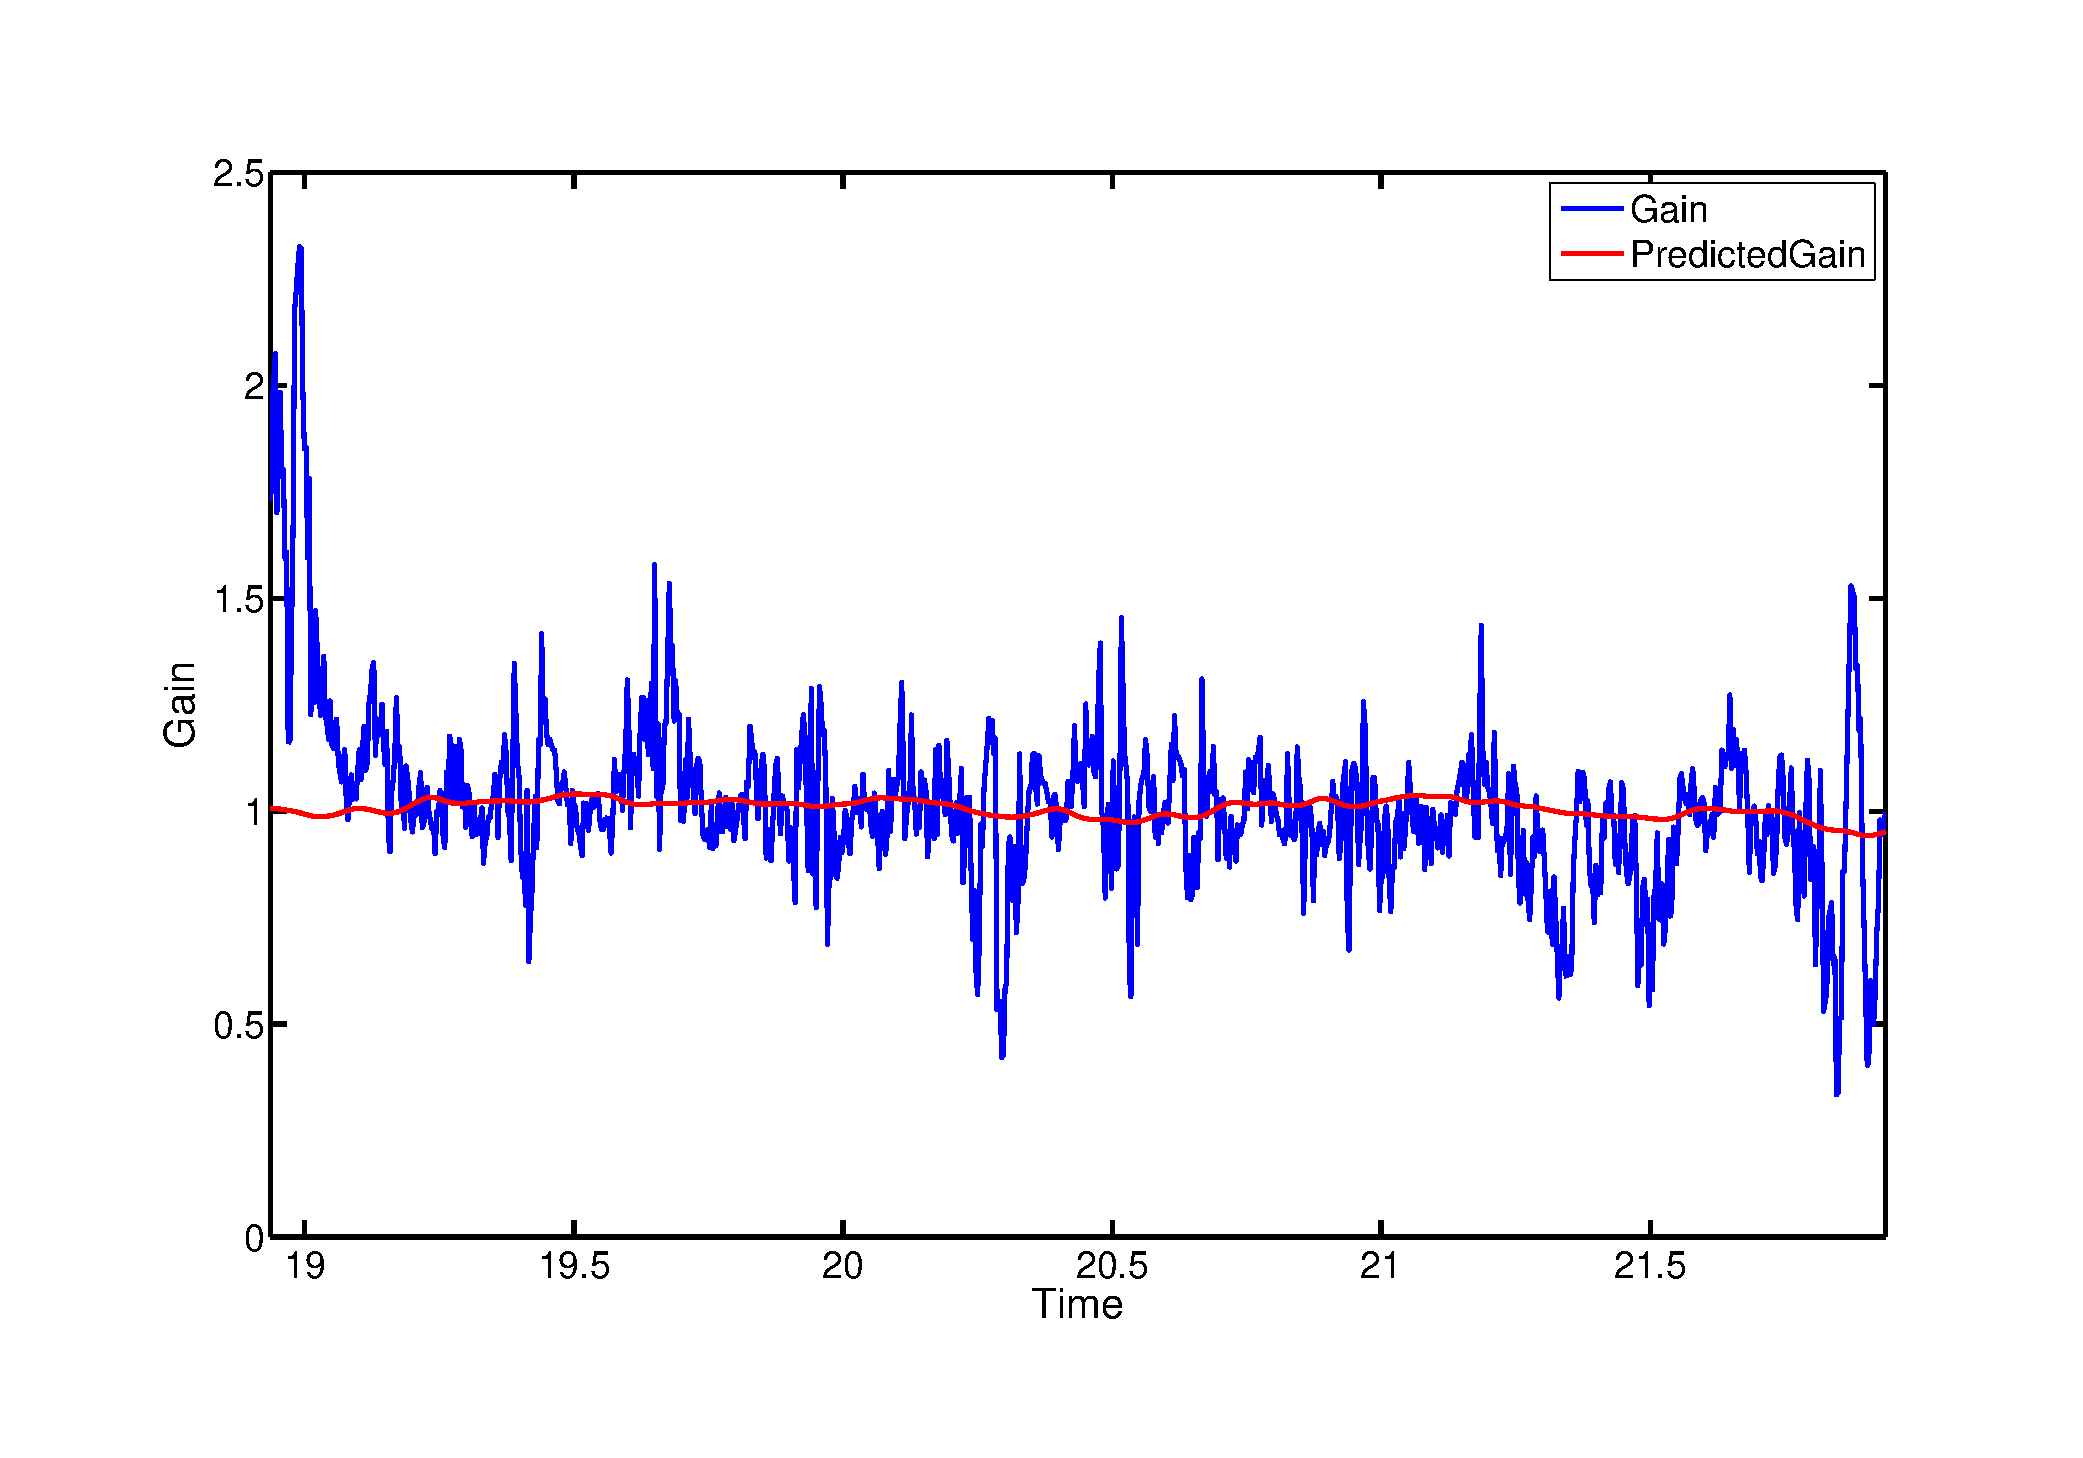
\includegraphics [width=\textwidth]{Analysis_January_15.pdf}
\begin{par}
Using this estimate, we can then correct the linear prediction of the firing rate.
\end{par} \vspace{1em}

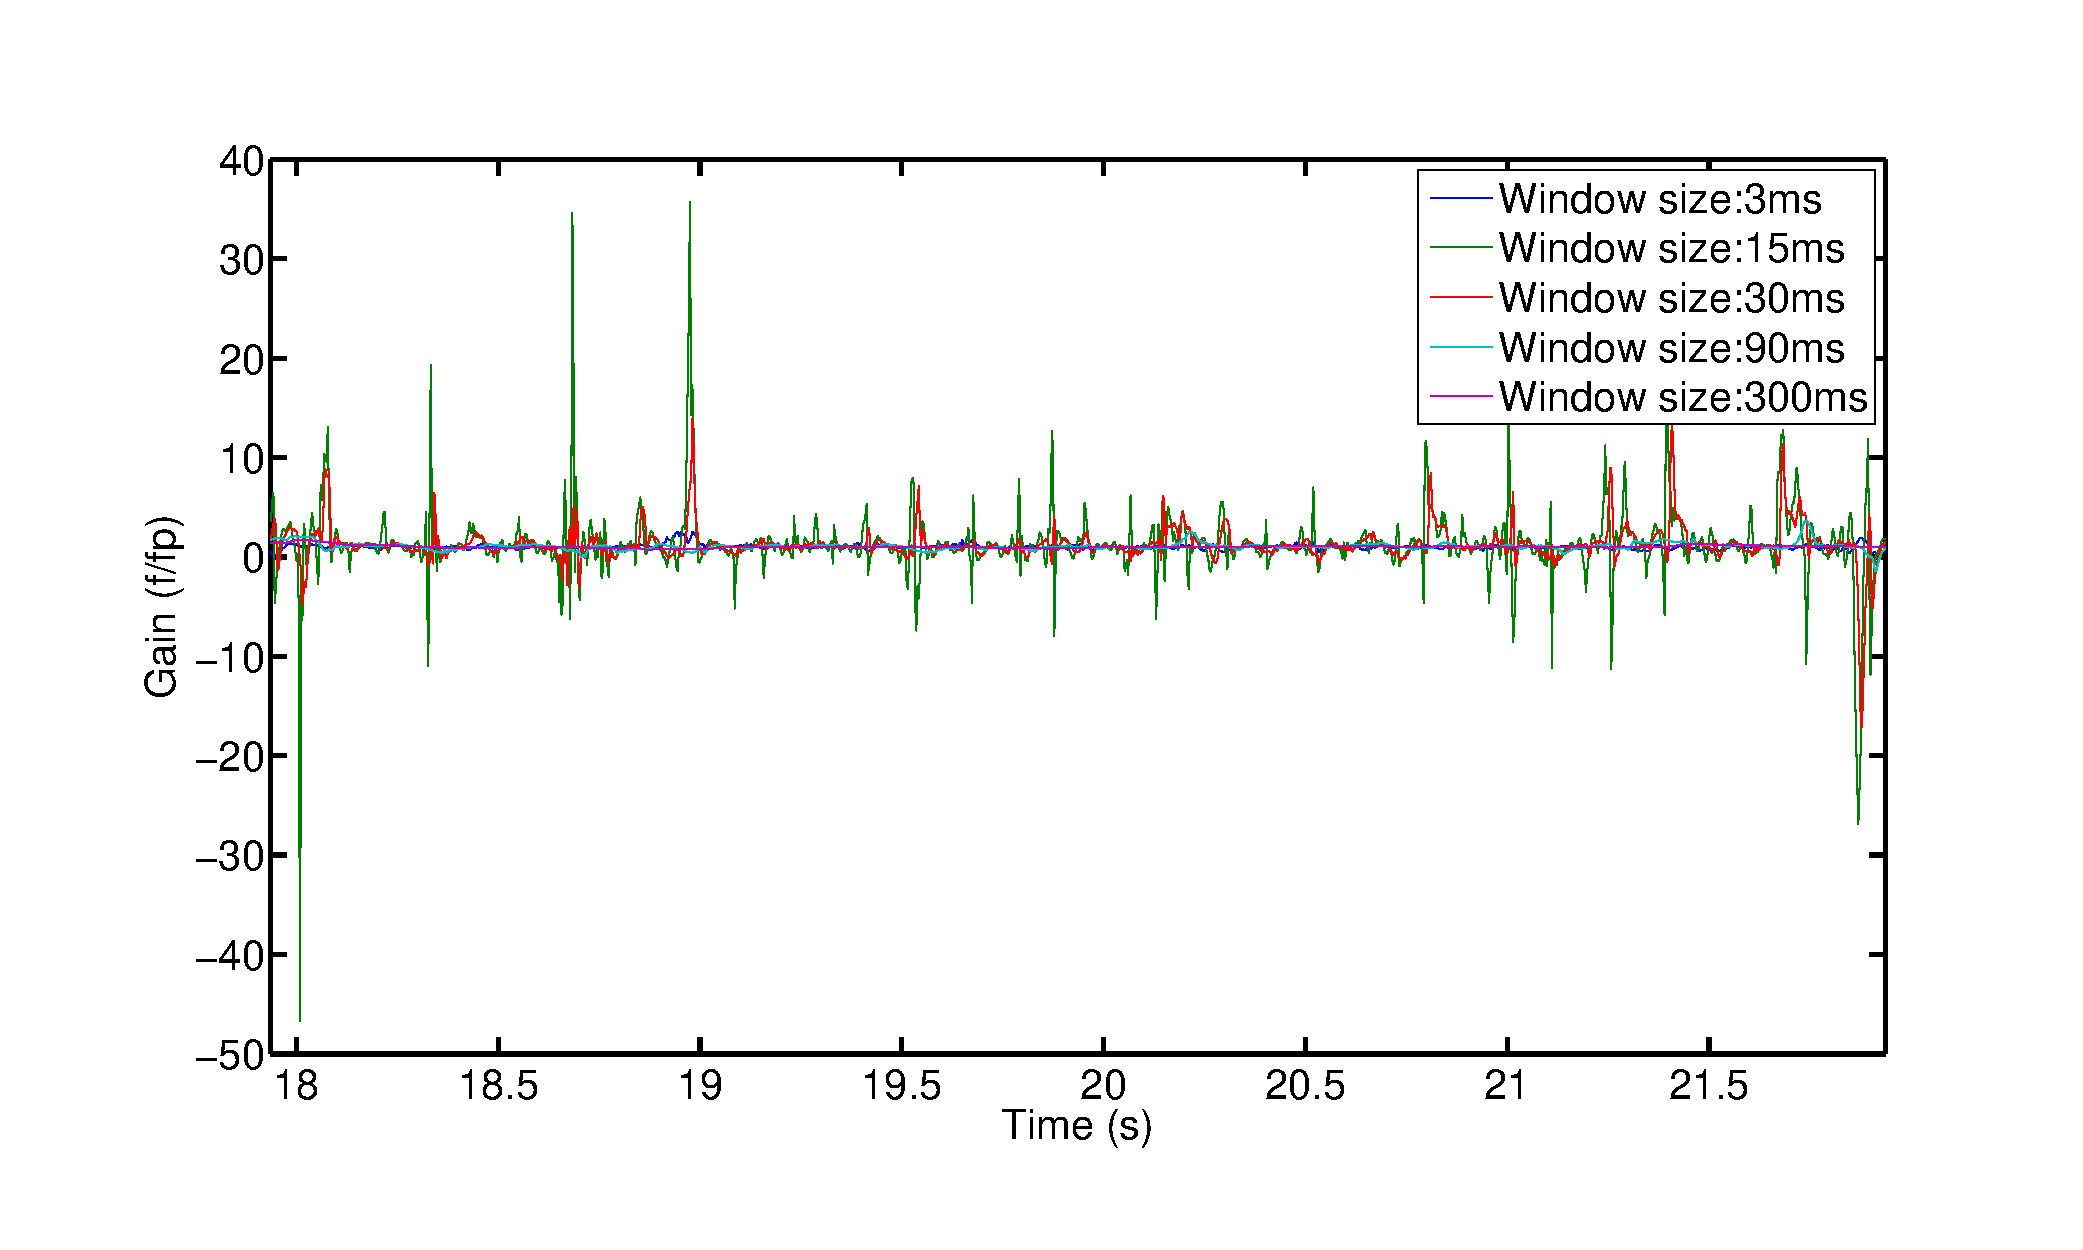
\includegraphics [width=\textwidth]{Analysis_January_16.pdf}
\begin{par}
Is the gain-corrected prediction any better than the linear prediction? The mean error of the gain-corrected prediction is
\end{par} \vspace{1em}

        \color{lightgray} \begin{verbatim}    1.4535

\end{verbatim} \color{black}
    \begin{par}
while the mean error of the simple linear prediction is
\end{par} \vspace{1em}

        \color{lightgray} \begin{verbatim}    1.3089

\end{verbatim} \color{black}
    \begin{par}
No matter what I do, I can't get use a linear filter to predict the gain well from the stimulus.
\end{par} \vspace{1em}
\begin{par}
The autocorrelation function of the gain shows that it is very tightly constrained, almost as much as the valve, and much less than the PID, which we are trying to use to predict it.
\end{par} \vspace{1em}

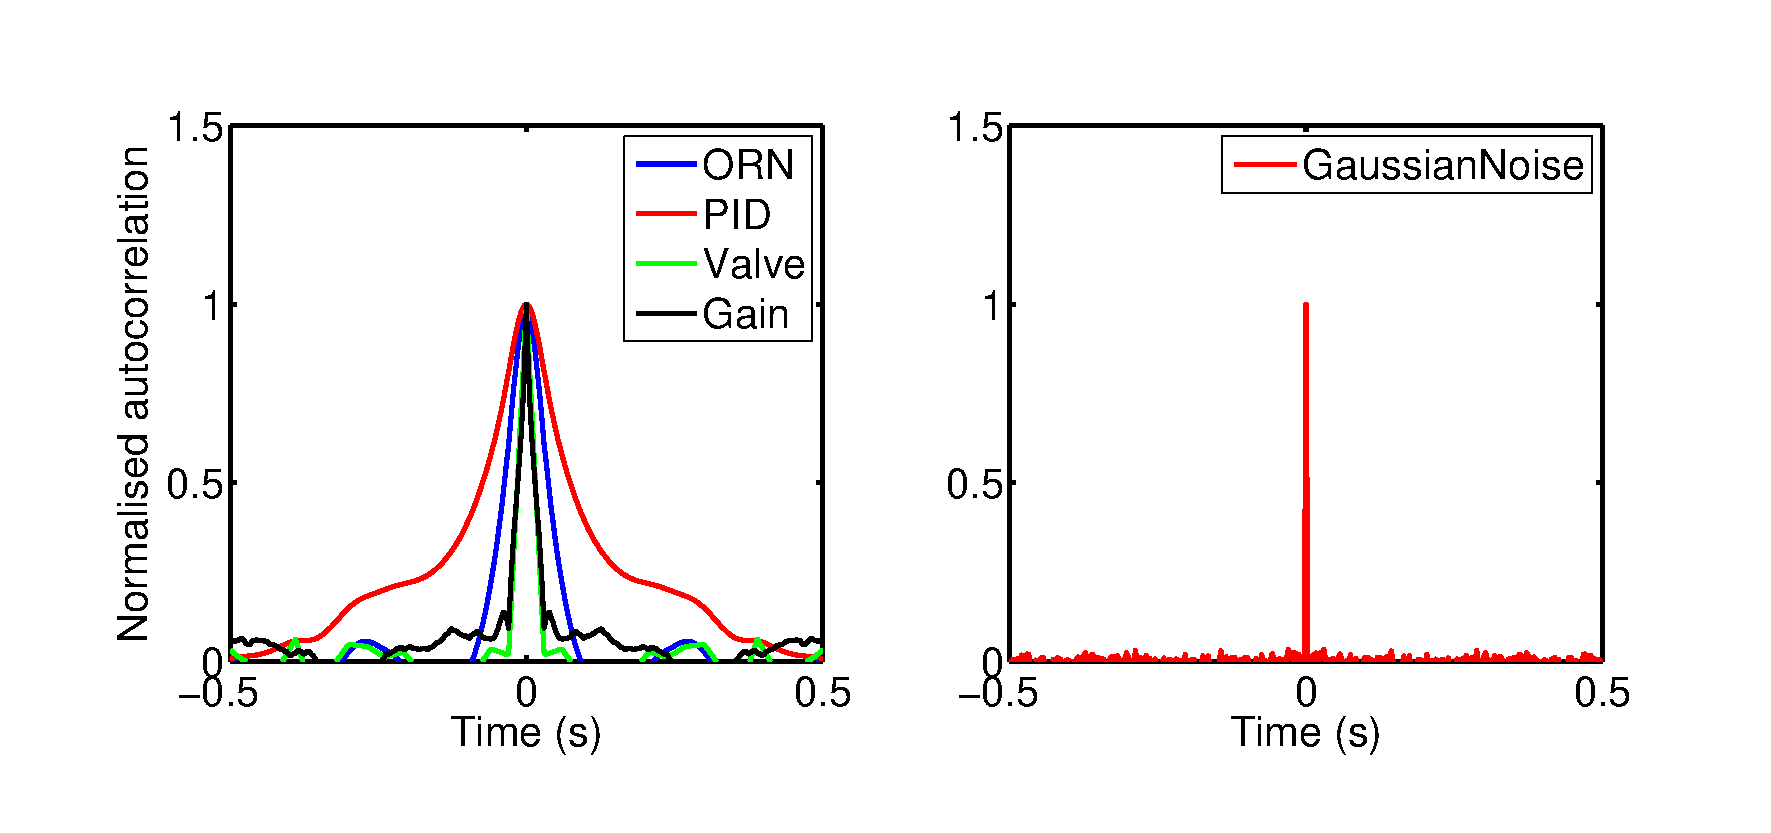
\includegraphics [width=\textwidth]{Analysis_January_17.pdf}


\subsection*{Summary/Problems}

\begin{enumerate}
\setlength{\itemsep}{-1ex}
   \item Best fit line of linear prediction to actual data does not have a slope of 1 for Damon's function. For synthetic data the slope of the line is indeed 1. However, in the real data set, it is not, even with no regularisation.
   \item Prediction of gain from past stimulus is very poor. The correlation coefficient of the prediction with the instantaneous gain is \ensuremath{\tilde{\;}} 0.2. For comparison, the corr. coeff. of the firing rate prediction \ensuremath{>} 0.95.
\end{enumerate}


\subsection*{Next Steps}

\begin{enumerate}
\setlength{\itemsep}{-1ex}
   \item Calculate filters for high and low stimulus zones.
   \item Calculate filters after using elastic net regularisation.
   \item Check if someone has looked at Weber's law in olfaction/ORNs
   \item shuffle data to check validity?
   \item fit Dynamical Adaptation model to data?
\end{enumerate}



\end{document}
    
